%%
%% 研究報告用スイッチ
%% [techrep]
%%
%% 欧文表記無しのスイッチ(etitle,eabstractは任意)
%% [noauthor]
%%

%\documentclass[submit,techrep]{ipsj}
%%% <<< SES
%\documentclass[submit,techrep,noauthor]{ipsj}
\documentclass[submit,ses,noauthor]{ipsj}
%%% >>> SES


\usepackage[dvips]{graphicx}
\usepackage{latexsym}
\usepackage{url}

\def\Underline{\setbox0\hbox\bgroup\let\\\endUnderline}
\def\endUnderline{\vphantom{y}\egroup\smash{\underline{\box0}}\\}
\def\|{\verb|}
%

%\setcounter{巻数}{59}%vol59=2018
%\setcounter{号数}{10}
%\setcounter{page}{1}


\begin{document}


\title{Scratchにおけるユーザの\\コンピュテーショナル・シンキング獲得過程\\に基づく
習熟度到達予測}

\etitle{Predicting Level Attainment Based on \\ Users' Computational Thinking Acquisition Process in Scratch }

\affiliate{IPSJ}{情報処理学会\\
IPSJ, Chiyoda, Tokyo 101--0062, Japan}


\paffiliate{JU}{情報処理大学\\
Johoshori Uniersity}

\author{岡本 圭悟}{Keigo Okamoto}{IPSJ}[joho.taro@ipsj.or.jp]
\author{伊原 彰紀}{Akinori Ihara}{IPSJ}

\begin{abstract}
本研究では,Scratchにおけるユーザのコンピュテーショナル・シンキング(CT)の作品制作過程に合わせた作品推薦に向けて,ユーザが予測時点でCT習熟度が向上する作品を制作するか否かを予測する手法を提案する.
Scratchでは,視覚的に表現されたブロックを組み合わせてプログラムを実装し,作品制作を通してCTを身につける.特に,ユーザは学習支援ツールDr.Scratchを使用することで,自身のCTスキルを定量的に把握できる.
従来研究では,ユーザが過去に獲得したCTスキルから,特定のCT習熟度への到達可否を予測するモデルを構築,評価した.しかし,従来モデルではユーザの作品制作過程は十分考慮できておらず,誤って予測することがある.
本研究では,まずユーザが獲得してきたCT7概念の特徴量を分析し,ユーザの作品制作過程を説明変数とした学習モデルを構築し,従来モデルとの比較評価を行った.
\end{abstract}


%
%\begin{jkeyword}
%情報処理学会論文誌ジャーナル,\LaTeX,スタイルファイル,べからず集
%\end{jkeyword}
%
%\begin{eabstract}
%This document is a guide to prepare a draft for submitting to IPSJ
%Journal, and the final camera-ready manuscript of a paper to appear in
%IPSJ Journal, using {\LaTeX} and special style files.  Since this
%document itself is produced with the style files, it will help you to
%refer its source file which is distributed with the style files.
%\end{eabstract}
%
%\begin{ekeyword}
%IPSJ Journal, \LaTeX, style files, ``Dos and Dont's'' list
%\end{ekeyword}

\maketitle

%1
\section{はじめに}
%%%%%%%%%%%%%%%%%%%%%%
ビジュアルプログラミング言語Scratch\cite{Resnick_2009}では,プログラミングにおける命令処理を視覚的なブロックとして表現し,それらを組み合わせることでプログラムが実装できる.また,ScratchはWeb上にオンライン学習サービス\footnote{Scratch: \url{https://scratch.mit.edu/}}を展開しており,ユーザは他ユーザが制作した作品を参照することが可能である.

ユーザはScratch上で作品制作を通してプログラミングに必要な能力であるコンピュテーショナル・シンキング(CT)を身につける.Scratch上でCTを定量的に把握できるツールとして,MorenoらはDr.Scratch~\cite{Moreno_2015}を開発している.Dr.Scratchは,Scratchプログラムから,作品の機能実装に必要な7つのCT概念をそれぞれ0点から3点までで算出し,合計点数0点から21点で作品を評価する.特に,CTスキルの区分としてCT習熟度が存在し,0点から7点をBasic,8点から14点をDeveloping,15点から21点をMasterとしている.

従来研究として安東ら~\cite{Ando_2021}はユーザのCTに合わせた作品推薦に向けて,ユーザが過去に制作した作品のCTスキルに基づいてユーザが次にCT習熟度が向上するかを予測する研究を行なった.しかし,従来モデルではユーザの作品製制作過程は十分考慮できておらず誤って予測することがある.このことから作品制作過程を考慮したモデルを構築することで,従来モデルで予測できなかった作品制作過程が類似するユーザの習熟度到達予測が可能になると考える.


\section{RQ1:CT習熟度が向上した多くのユーザが獲得してきたCT7概念の違いはどの程度か?}\label{sec:chapter_3}
\section{概要}
本章では,作品制作の過程でCT習熟度が向上したユーザに焦点を当て,各ユーザが獲得してきたCT7概念の特徴を明らかにする.

従来研究では,ユーザがCT習熟度を向上させる過程でどのようなCTスキルを獲得しているかは詳細に分析されていない.習熟度が向上するまでにユーザが獲得してきたCT7概念(CTパス)の違いを明らかにするために,ユーザの習熟度が向上する地点までの作品におけるCT7概念を計測する.また,CT習熟度が向上するまでに制作した作品の数やCTパスの重複数を基に,作品制作過程とCT概念の特徴をそれぞれ分析する.


\section{データセット}\label{sec:chapter_3-1}
従来研究では,ユーザが共通の開発環境で制作した作品を比較するため,バージョン3.0をリリースした2019年1月3日から2020年1月3日までの間に初めて作品公開を行ったユーザを分析対象とし,サービス上に20件以上の作品を公開しているユーザ7,050人が制作した作品141,000件(7,050人×20件)を収集した.本研究ではそれらの作品をDr.ScratchによりCTスコアの計測を行い,失敗しなかった作品を制作したユーザ6,323人が1番目から20番目までに制作した作品126,460件を本分析の対象とする.


\section{分析手法}\label{sec:chapter_3-2}
従来研究~\cite{Ando_2021}ではユーザが一度でも特定の習熟度を満たす作品を制作すれば当該習熟度に到達したと判断しており,リミックス作品による獲得は習熟度到達として認めていない.本研究では,従来研究の設定と同様に,20番目の作品を制作するまでにBasicからDeveloping以上に向上したユーザ(BtoDユーザ)3,125人,DevelopingからMasterに向上したユーザ(DtoMユーザ)1,196人を分析対象とする.また,20番目の作品を制作する過程で,BasicからDevelopingに向上し,さらにDevelopingからMasterに向上するユーザもいるため,BtoDユーザとDtoMユーザの間には重複がある.

本分析では,BtoDユーザとDtoMユーザそれぞれについて,習熟度が向上するまでに獲得したCT7概念の系列(CTパス)を抽出する.リミックス作品も学習の一部とみなし,習熟度向上の過程で制作されたリミックス作品もCTパスに含める.

図\ref{fig:digraph}は2人のBtoDユーザのCTパスの事例を状態遷移図として示す.図中のノードは,制作された作品から測定されたCT7概念のスコア分布を示し,次に制作する作品へのつながりはエッジで表現する.各ノード内のレーダーチャートのラベル記号は,対応するCT7概念に一致し,表\ref{tab:ct-symobol}にその対応関係を示す.各項目はチャートの最外側が3点,最内側が0点とする.図\ref{fig:digraph}のBtoDユーザAは最初に全てのCTスコアが0点の作品を制作し,次にフロー制御,ユーザ対話性,データ表現の概念を1点を獲得した後,ユーザ対話性と論理の概念で2点向上させ,習熟度Developingに到達している.

多くのユーザが経由する作品制作過程の特徴を分析するため,各ユーザがCT習熟度が向上するまでに制作した作品数と,BtoDユーザ,DtoMユーザ毎のエッジの重複数を算出する.例えば,図\ref{fig:digraph}のユーザAは習熟度が向上するまでに制作した作品数が3であり,ユーザBは2である.また,ノード$A_1$とノード$B_1$,ノード$A_2$とノード$B_2$で制作された作品は同じCT概念を用いているため,CTパスが重複している.ユーザの作品制作過程の再現性を確認するため,ユーザのCTパス重複数として,ユーザのCTパスの各エッジの重複数を合計し,エッジ数で割った平均値を用いる.ユーザAとユーザBのみを分析する場合,ユーザAの各エッジの重複数は1,2,2となり,ユーザAのCTパス重複数は$(1 + 2 + 2) / 3 = 1.67$となる.

本分析では,より特徴のあるCTパスを抽出するため,習熟度を向上させる際に制作した作品のCT概念の重複数が多いユーザに着目する.また,ユーザが習熟度向上までにかかる時間による違いも明らかにするため,習熟度向上までに制作した作品数毎のCTパス(代表CTパス)を抽出する.代表CTパスは習熟度向上までに制作した作品数毎に取得したCTパスに対し,以下の操作を行なって抽出する.
\begin{enumerate}
    \item 習熟度向上までに制作した作品数毎に各エッジの重複数を算出する.
    \item 習熟度向上の際に作成した作品から最大のエッジの重複数を持つノードに移る.
    \item 現在のノードの直前にある最大のエッジの重複数を持つノードを確認する.
    \item 最大のエッジの重複数を持つノードが一つしか存在しなかった場合そのノードに移り,3の操作を行う.複数ある場合は5の操作を行う.現在のノードが初期ノードである場合,6の操作を行う.
    \item ユーザ全体のCTパスから各エッジの重複数(重要度)を算出し,4で特定した複数のエッジの中から,重要度が最も高いエッジの重複数を持つノードに移り,3の操作を行う.現在のノードが初期ノードである場合,6の操作を行う.
    \item 現在のノードまでに辿ってきたパスを代表CTパスとして抽出する.
\end{enumerate}



\begin{figure*}[t]
	\centering
	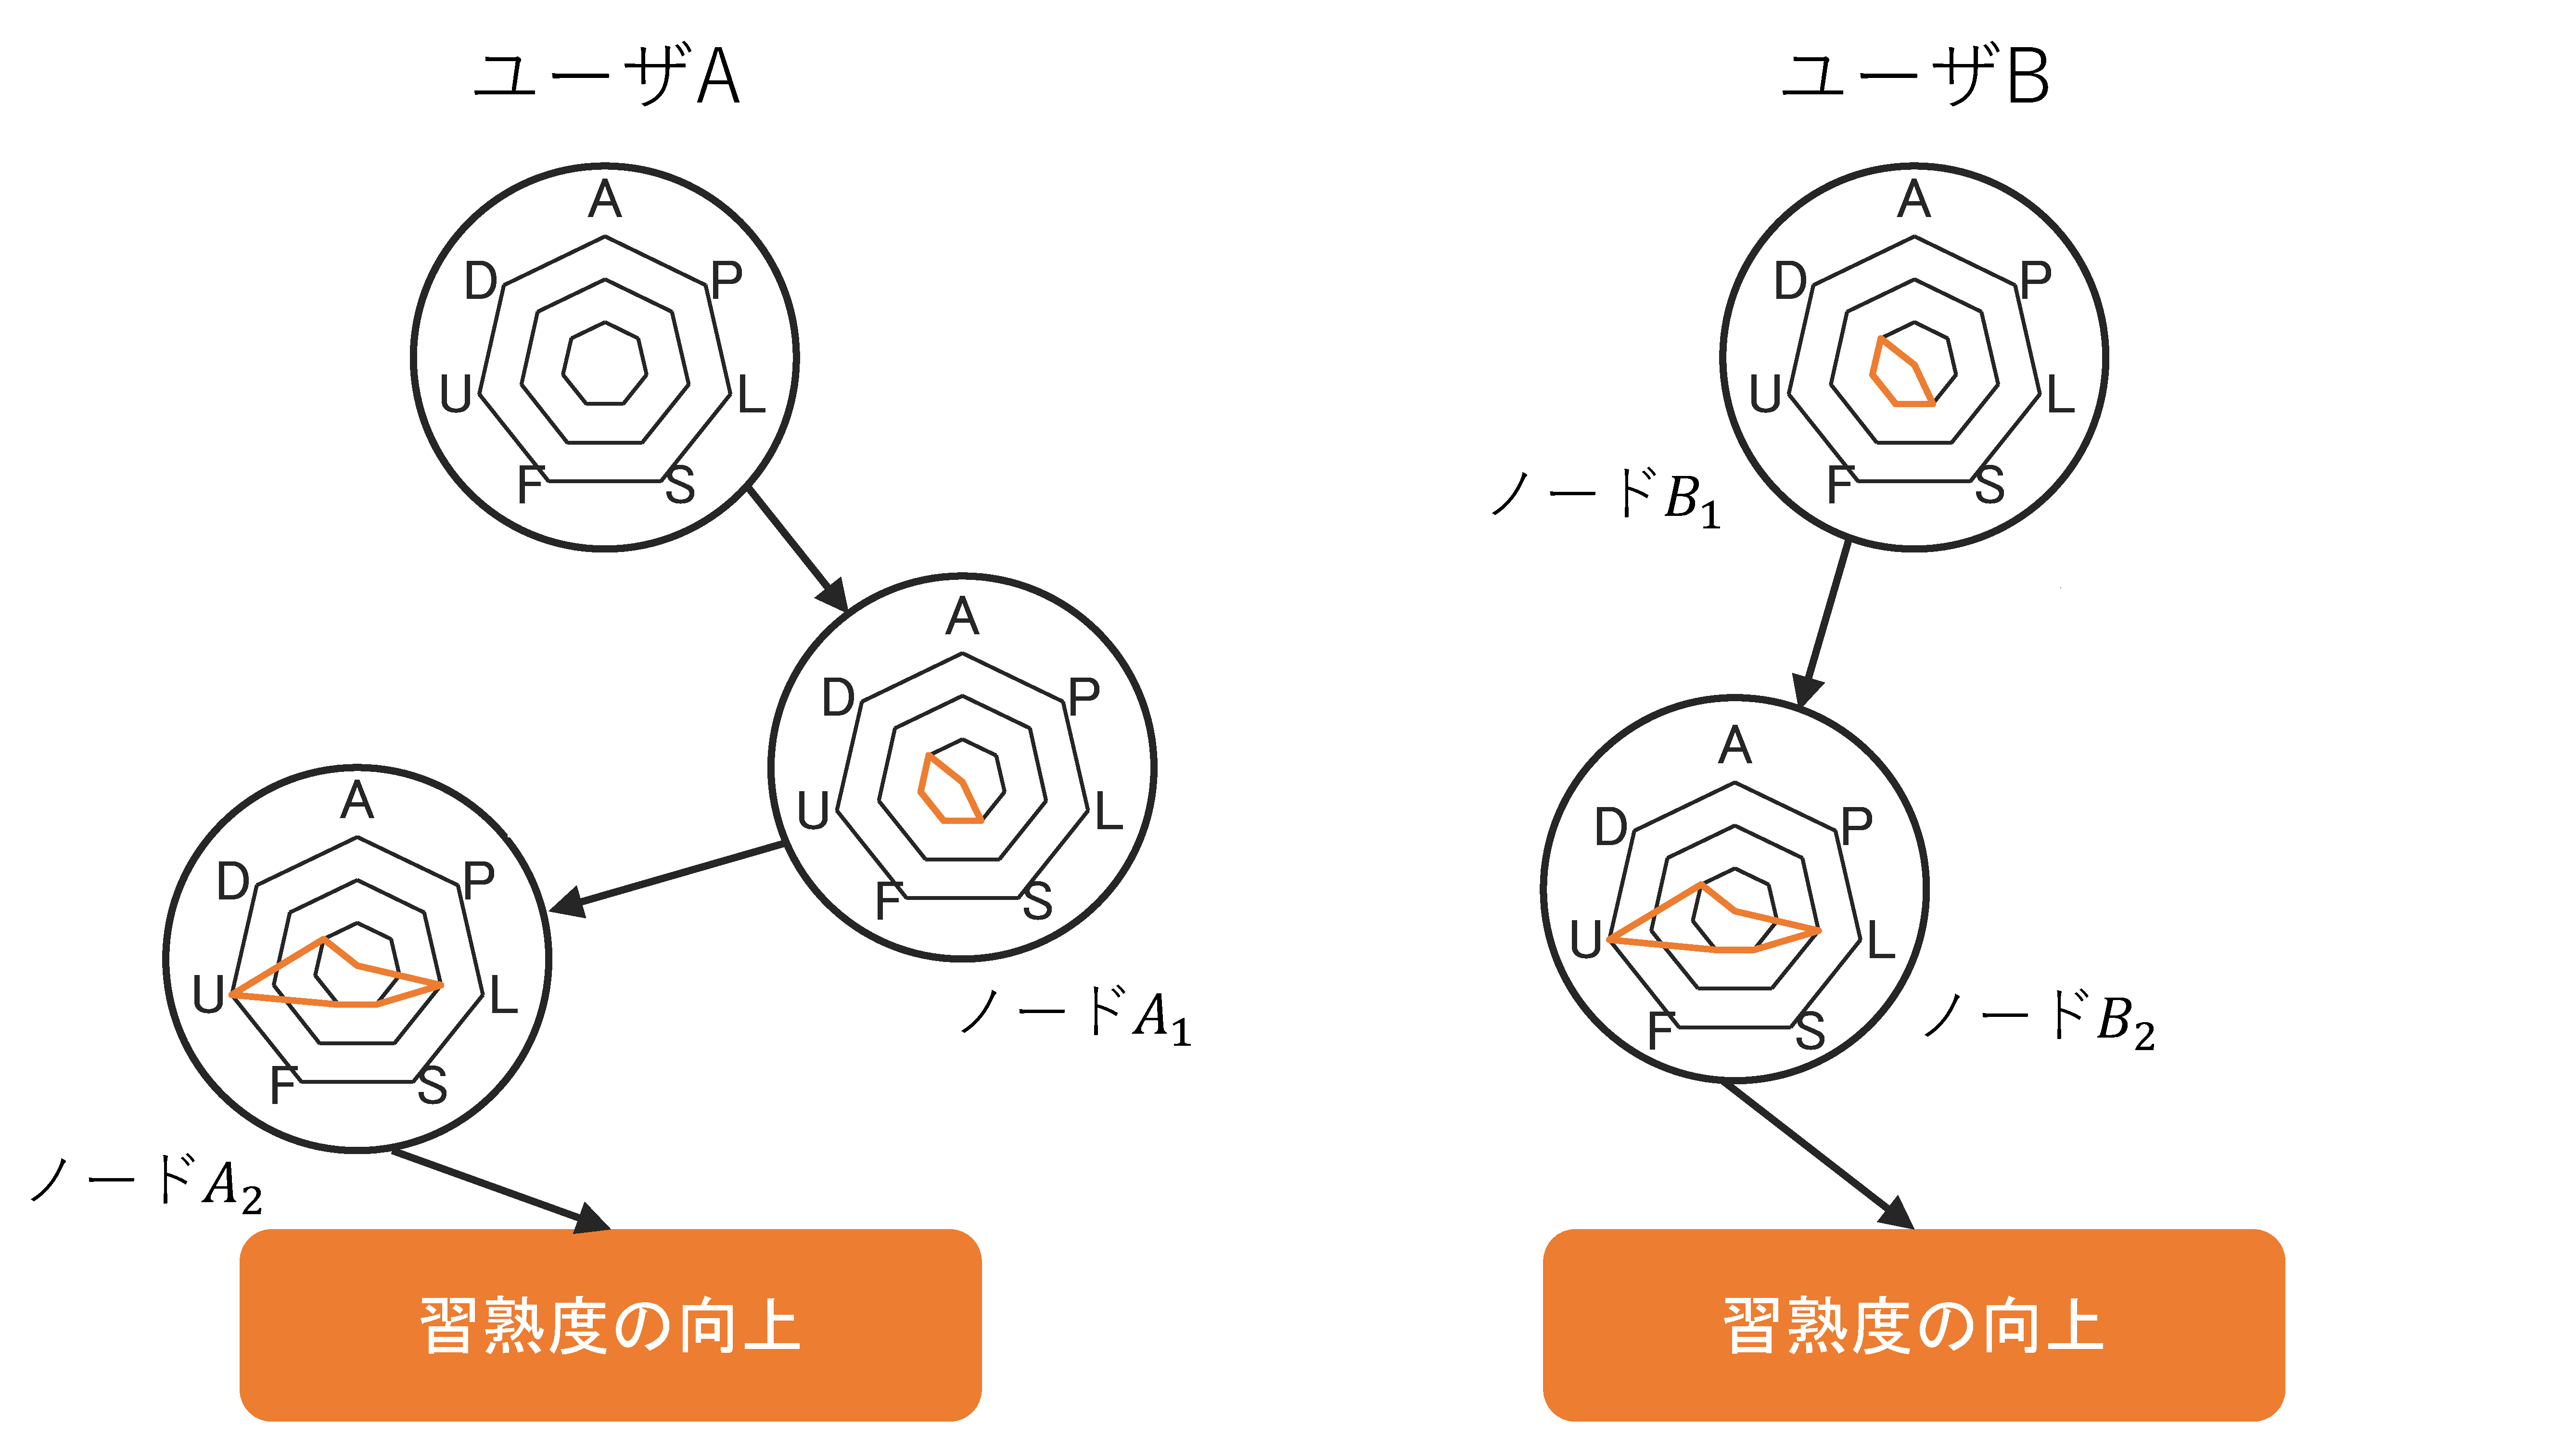
\includegraphics[width=1.0\linewidth]{Okamoto_fig/digraph.pdf}
	\caption{BtoDユーザ二人のCTパスを示した状態遷移図}
	\label{fig:digraph}
\end{figure*}

\begin{table}
  \caption{記号とCT7概念の対応表}
  \label{tab:ct-symobol}
  \vspace{2mm}
  \centering
  \begin{tabular}{c|c}
    \hline
    記号 & CT7概念\\
    \hline
    \hline
    A & 抽象化 \\
    \hline
    P & 並列 \\
    \hline
    S & 同期 \\
    \hline
    L & 論理 \\
    \hline
    F & フロー制御 \\
    \hline
    U & ユーザ対話性 \\
    \hline
    D & データ表現 \\
    \hline
  \end{tabular}
\end{table}




\section{分析結果}\label{sec:3-analysis}
\subsection{作品制作過程の特徴量分析}\label{subsec:path-analysis}
図\ref{fig:dupli-mean}は各習熟度レベルへ向上したユーザのCTパスの重複数を示す箱ひげ図である.BtoDユーザのCTパスの重複数に関して,中央値が10.5,平均値が35.8であることから,BasicからDeveloping以上のレベルに習熟度が到達するユーザは,再現性のあるCTパスをたどって習熟度を向上させていることがわかる.一方,DtoMユーザのCTパスの重複数においては,中央値が1.0,平均値が2.4となっており,DevelopingからMasterレベルに習熟度を向上させるユーザは,より多様なCTパスを経由して習熟度を向上させていることが示されている.BtoDユーザとDtoMユーザ間でMann-Whitney U検定\cite{Mann1947OnAT}を適用した結果,統計的に有意差(p値$<$0.05)が確認されたことから,BtoDユーザとDtoMユーザが異なるCTパスを辿って習熟度を向上させていることを示している.

また,図\ref{fig:path-length}は各習熟度レベルに向上するまでにユーザが制作する作品数の分布を示す箱ひげ図である.BtoDユーザが習熟度を向上させるまでに制作する作品数の中央値は6.0,平均値は7.2であり,DtoMユーザのそれは中央値が10.0,平均値が9.6であった.BtoDユーザとDtoMユーザ間でMann-Whitney U検定を実施したところ,統計的に有意な差(p値$<$0.05)が見られたことから,習熟度を向上させる過程で必要とする作品数にはグループ間で差があり,BtoDユーザはDtoMユーザに比べてより短期間で特定の習熟度に到達している.

\begin{figure*}[t]
	\centering
	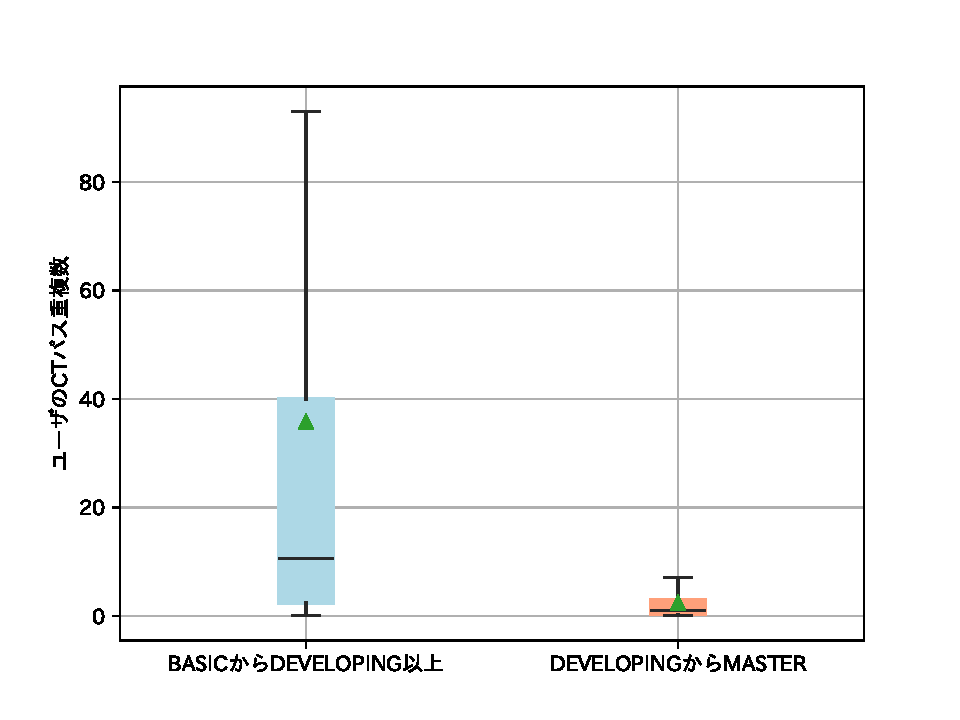
\includegraphics[width=0.8\linewidth]{Okamoto_fig/dupli-all.pdf}
        \vspace{-5mm}
	\caption{各習熟度に到達したユーザのCTパス重複数平均値の分布}
	\label{fig:dupli-mean}
\end{figure*}

\begin{figure*}[t]
	\centering
	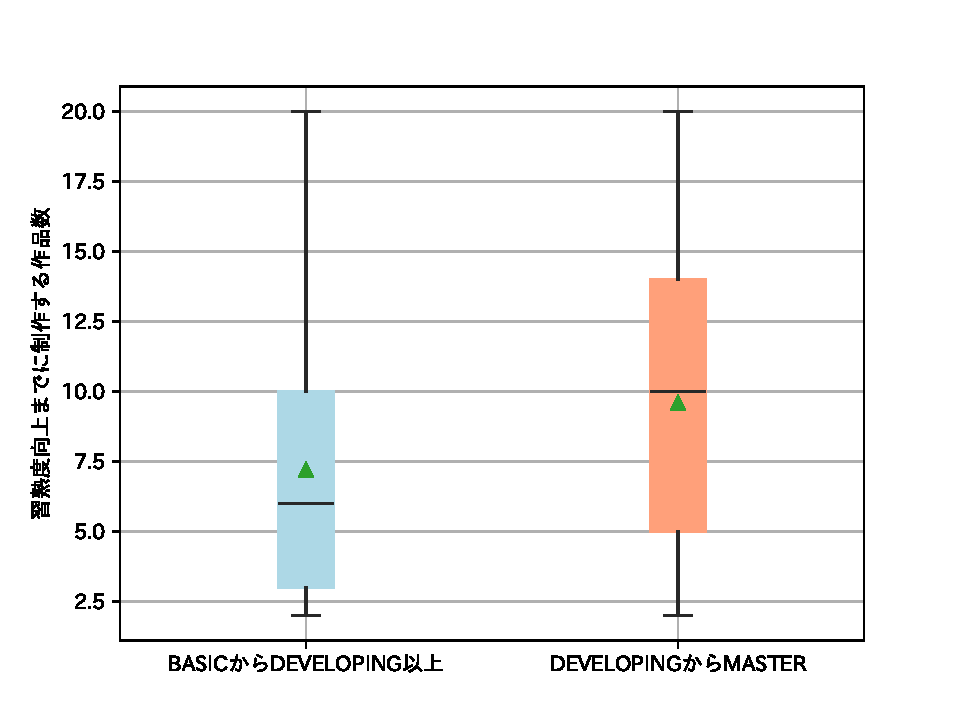
\includegraphics[width=0.8\linewidth]{Okamoto_fig/path-length.pdf}
        \vspace{-5mm}
	\caption{各習熟度に到達したユーザが習熟度向上までに制作する作品数の分布}
	\label{fig:path-length}
\end{figure*}

\subsection{CT獲得過程の分析}\label{subsec:ct-analysis}

表\ref{tab:ranking-btod}にBtoDユーザの中で,習熟度を向上させる際に制作した作品のCT概念の重複数が上位10件にランクされたユーザを示す.CT概念に用いている記号は\ref{sec:chapter_3-2}節で用いた表\ref{tab:ct-symobol}と対応している.データセットから抽出した全BtoDユーザ3,125人の中で,表\ref{tab:ranking-btod}に示す上位10件のCT概念を使用する作品制作したユーザ数は1,209人(約39\%)である.この1,209人の各CT概念において,全ユーザが抽象化で1点を獲得しており,8位を除く全てでデータ表現のスキルを1点獲得している.つまり,多くのBtoDユーザが最終的に抽象化とデータ表現のスキルを獲得していることを示している.

\begin{table}[]
\caption{BtoDユーザが習熟度向上の際に制作する作品のCTスコア重複数の上位10件}
  \label{tab:ranking-btod}
  \vspace{2mm}
  \centering
\begin{tabular}{c|c|cccccccc}
\hline
\multirow{2}{*}{順位} & \multirow{2}{*}{ユーザ数} & \multicolumn{8}{c}{CTスコア}                                                                                               \\ \cline{3-10} 
                    &                      & \multicolumn{1}{c|}{抽象化}  & \multicolumn{1}{c|}{並列} & \multicolumn{1}{c|}{論理} & \multicolumn{1}{c|}{同期} & \multicolumn{1}{c|}{フロー制御} & \multicolumn{1}{c|}{ユーザ対話性} & \multicolumn{1}{c|}{データ表現} & 合計 \\ \hline
                    \hline
1                   & 291                  & \multicolumn{1}{c|}{1} & \multicolumn{1}{c|}{2} & \multicolumn{1}{c|}{0} & \multicolumn{1}{c|}{1} & \multicolumn{1}{c|}{2} & \multicolumn{1}{c|}{2} & \multicolumn{1}{c|}{1} & 9  \\ \hline
2                   & 227                  & \multicolumn{1}{c|}{1} & \multicolumn{1}{c|}{2} & \multicolumn{1}{c|}{0} & \multicolumn{1}{c|}{0} & \multicolumn{1}{c|}{2} & \multicolumn{1}{c|}{2} & \multicolumn{1}{c|}{1} & 8  \\ \hline
3                   & 154                  & \multicolumn{1}{c|}{1} & \multicolumn{1}{c|}{1} & \multicolumn{1}{c|}{0} & \multicolumn{1}{c|}{1} & \multicolumn{1}{c|}{2} & \multicolumn{1}{c|}{2} & \multicolumn{1}{c|}{1} & 8  \\ \hline
4                   & 118                  & \multicolumn{1}{c|}{1} & \multicolumn{1}{c|}{2} & \multicolumn{1}{c|}{0} & \multicolumn{1}{c|}{1} & \multicolumn{1}{c|}{1} & \multicolumn{1}{c|}{2} & \multicolumn{1}{c|}{1} & 8  \\ \hline
5                   & 107                  & \multicolumn{1}{c|}{1} & \multicolumn{1}{c|}{1} & \multicolumn{1}{c|}{1} & \multicolumn{1}{c|}{0} & \multicolumn{1}{c|}{2} & \multicolumn{1}{c|}{2} & \multicolumn{1}{c|}{1} & 8  \\ \hline
6                   & 82                   & \multicolumn{1}{c|}{1} & \multicolumn{1}{c|}{1} & \multicolumn{1}{c|}{0} & \multicolumn{1}{c|}{2} & \multicolumn{1}{c|}{2} & \multicolumn{1}{c|}{1} & \multicolumn{1}{c|}{1} & 8  \\ \hline
7                   & 67                   & \multicolumn{1}{c|}{1} & \multicolumn{1}{c|}{3} & \multicolumn{1}{c|}{0} & \multicolumn{1}{c|}{2} & \multicolumn{1}{c|}{2} & \multicolumn{1}{c|}{1} & \multicolumn{1}{c|}{1} & 10 \\ \hline
8                   & 60                   & \multicolumn{1}{c|}{1} & \multicolumn{1}{c|}{1} & \multicolumn{1}{c|}{1} & \multicolumn{1}{c|}{0} & \multicolumn{1}{c|}{2} & \multicolumn{1}{c|}{2} & \multicolumn{1}{c|}{2} & 9  \\ \hline
9                   & 52                   & \multicolumn{1}{c|}{1} & \multicolumn{1}{c|}{3} & \multicolumn{1}{c|}{0} & \multicolumn{1}{c|}{3} & \multicolumn{1}{c|}{1} & \multicolumn{1}{c|}{1} & \multicolumn{1}{c|}{1} & 10 \\ \hline
10                  & 51                   & \multicolumn{1}{c|}{1} & \multicolumn{1}{c|}{3} & \multicolumn{1}{c|}{0} & \multicolumn{1}{c|}{2} & \multicolumn{1}{c|}{1} & \multicolumn{1}{c|}{1} & \multicolumn{1}{c|}{1} & 9 \\ \hline
\end{tabular}
\end{table}

表\ref{tab:ranking-dtom}にDtoMユーザの中で,習熟度を向上させる際に制作した作品のCT概念の重複数が上位10件にランクされたユーザを示す.CT概念に用いている記号は\ref{sec:chapter_3-2}節で用いた表\ref{tab:ct-symobol}と対応している.データセットから抽出した全DtoMユーザ1,196人の中で,表\ref{tab:ranking-dtom}に示す上位10件のCT概念を使用する作品制作したユーザ数は523人(約44\%)であった.この523人の各CT概念において,全ユーザがユーザ対話性とデータ表現のスキルで2点を獲得しており,10位を除く全てで並列処理のスキルを3点獲得している.これは,多くのDtoMユーザが最終的にユーザ対話性,データ表現,並列処理のスキルを獲得していることを示している.

\begin{table}[]
\caption{DtoMユーザが習熟度向上の際に制作する作品のCTスコア重複数の上位10件}
  \label{tab:ranking-dtom}
  \vspace{2mm}
  \centering
\begin{tabular}{c|c|cccccccc}
\hline
\multirow{2}{*}{順位} & \multirow{2}{*}{ユーザ数} & \multicolumn{8}{c}{CTスコア}                                                                                                                                                         \\ \cline{3-10} 
                    &                      & \multicolumn{1}{c|}{抽象化} & \multicolumn{1}{c|}{並列} & \multicolumn{1}{c|}{論理} & \multicolumn{1}{c|}{同期} & \multicolumn{1}{c|}{フロー制御} & \multicolumn{1}{c|}{ユーザ対話性} & \multicolumn{1}{c|}{データ制御} & 合計 \\ \hline \hline
1                   & 112                  & \multicolumn{1}{c|}{3} & \multicolumn{1}{c|}{3} & \multicolumn{1}{c|}{3} & \multicolumn{1}{c|}{3} & \multicolumn{1}{c|}{3} & \multicolumn{1}{c|}{2} & \multicolumn{1}{c|}{2} & 19  \\ \hline
2                   & 84                  & \multicolumn{1}{c|}{1} & \multicolumn{1}{c|}{3} & \multicolumn{1}{c|}{3} & \multicolumn{1}{c|}{2} & \multicolumn{1}{c|}{2} & \multicolumn{1}{c|}{2} & \multicolumn{1}{c|}{2} & 15  \\ \hline
3                   & 74                  & \multicolumn{1}{c|}{1} & \multicolumn{1}{c|}{3} & \multicolumn{1}{c|}{3} & \multicolumn{1}{c|}{3} & \multicolumn{1}{c|}{2} & \multicolumn{1}{c|}{2} & \multicolumn{1}{c|}{2} & 16  \\ \hline
4                   & 56                  & \multicolumn{1}{c|}{1} & \multicolumn{1}{c|}{3} & \multicolumn{1}{c|}{3} & \multicolumn{1}{c|}{3} & \multicolumn{1}{c|}{3} & \multicolumn{1}{c|}{2} & \multicolumn{1}{c|}{2} & 17  \\ \hline
5                   & 55                  & \multicolumn{1}{c|}{1} & \multicolumn{1}{c|}{3} & \multicolumn{1}{c|}{2} & \multicolumn{1}{c|}{3} & \multicolumn{1}{c|}{2} & \multicolumn{1}{c|}{2} & \multicolumn{1}{c|}{2} & 15  \\ \hline
6                   & 31                   & \multicolumn{1}{c|}{1} & \multicolumn{1}{c|}{3} & \multicolumn{1}{c|}{2} & \multicolumn{1}{c|}{2} & \multicolumn{1}{c|}{3} & \multicolumn{1}{c|}{2} & \multicolumn{1}{c|}{3} & 16  \\ \hline
7                   & 29                   & \multicolumn{1}{c|}{1} & \multicolumn{1}{c|}{3} & \multicolumn{1}{c|}{1} & \multicolumn{1}{c|}{3} & \multicolumn{1}{c|}{3} & \multicolumn{1}{c|}{2} & \multicolumn{1}{c|}{2} & 15 \\ \hline
8                   & 28                   & \multicolumn{1}{c|}{1} & \multicolumn{1}{c|}{3} & \multicolumn{1}{c|}{3} & \multicolumn{1}{c|}{2} & \multicolumn{1}{c|}{3} & \multicolumn{1}{c|}{2} & \multicolumn{1}{c|}{2} & 16  \\ \hline
9                   & 27                   & \multicolumn{1}{c|}{3} & \multicolumn{1}{c|}{3} & \multicolumn{1}{c|}{3} & \multicolumn{1}{c|}{2} & \multicolumn{1}{c|}{3} & \multicolumn{1}{c|}{2} & \multicolumn{1}{c|}{2} & 18 \\ \hline
10                  & 27                   & \multicolumn{1}{c|}{3} & \multicolumn{1}{c|}{1} & \multicolumn{1}{c|}{3} & \multicolumn{1}{c|}{2} & \multicolumn{1}{c|}{3} & \multicolumn{1}{c|}{2} & \multicolumn{1}{c|}{2} & 16  \\ \hline
\end{tabular}
\end{table}

\subsubsection*{BtoDユーザの分析}

全BtoDユーザの中から表\ref{tab:ranking-btod}で1位であったユーザ291人を抽出し,習熟度向上までに制作した作品数毎の代表CTパスを抽出した結果を表\ref{tab:split-ct-btod}に示す.表\ref{tab:split-ct-btod}の代表CTパスは記号の羅列として表現されており,頻繁に利用される記号とCTスキルの対応表は表\ref{tab:dict-btod}に示す.例えば,作品数2の代表CTパスがBBであるため,この代表CTパスを通るユーザは抽象化,並列,同期,ユーザ対話性,データ表現で1点,フロー制御で2点を2作品連続で獲得したのち,Developingに到達する作品を制作している.

代表CTパスの中でも,特にBは作品制作数を跨いで8回出現している.これは代表CTパス中に含まれるCTスキルの中で最多の出現回数であり,BのCTスキル,つまり抽象化,並列,同期,ユーザ対話性,データ表現のスキルを1点,フロー制御のスキルを2点を獲得することがDevelopingへの向上につながることが示唆される.

表\ref{tab:split-ct-btod}の作品数2,3,7,8,10,11,12,13,15,18の代表CTパスでは,同じCT概念の作品を複数回連続して制作している.これは,ユーザが同じCT概念を連続で利用することで,習熟度の向上につながることを示唆している.作品数が10以下ではB,F,Jの点数を連続して獲得している一方で,作品数11以上ではN,L,Qを連続して獲得している.B,F,Jには共通してフロー制御が2点,ユーザ対話性とデータ表現が1点含まれる一方,N,L,Qには共通してフロー制御,ユーザ対話性,データ表現が1点ずつ含まれている.このことから,制作する作品数が異なっても,作品制作過程で獲得するCT概念は同じだが,点数が低い方が習熟度の向上に時間がかかることが示唆される.

また,作品数14,16,17の代表CTパスでは,部分的に同じCT概念を繰り返し獲得することで習熟度を向上させている.例えば,作品数14の代表CTパスでは,NBSのCT概念を4回とNBのCT概念を1回獲得したのちに習熟度を向上させている.繰り返して獲得しているCT概念のセットはNBS,UOQV,CYAである.NBSは共通してフロー制御,ユーザ対話性,データ表現を1点ずつ獲得しているセットである.UOQVは途中に二度Master以上のCTスコアを持つ作品をリミックスしている.CYAは4点以下の作品のみを制作し,途中には0点の作品も制作している.このことから,部分的に同じCT概念を繰り返し獲得するユーザのCTパスは,制作する作品数によってその特徴が異なることが示唆される.


\begin{table}[h]
  \begin{minipage}[t]{0.45\linewidth} % 0.5\linewidthはページ幅の半分に相当
    \centering
    \caption{対象BtoDユーザが習熟度向上までに制作した作品数毎の代表CTパス}
    \label{tab:split-ct-btod}
    \vspace{2mm}
  \begin{tabular}{c|l}
    \hline
    作品数 & 代表CTパス\\
    \hline
    \hline
    1 & A \\
    \hline
    2 & BB \\
    \hline
    3 & BBB \\
    \hline
    4 & ACDE \\
    \hline
    5 & FGHFI \\
    \hline
    6 & JBKLJM \\
    \hline
    7 & FFFFFFF  \\
    \hline
    8 & JJJJJJJM \\
    \hline
    9 & NNNHBKHJM \\
    \hline
    10 & BBBBBBBBBO \\
    \hline
    11 & NNNNNNNNPBI \\
    \hline
    12 & NNNNNNNNNNNN \\
    \hline
    13 & LLLLLLLLLLLQR \\
    \hline
    14 & NBSNBSNBSNBSNB \\
    \hline
    15 & QQQQQQQQQQQQQQT \\
    \hline
    16 & UOQVWUOQVWUOQVXB \\
    \hline
    17 & CYACYACYACYACYACZ \\
    \hline
    18 & NNNNNNNNNNNNNNNNNN \\
    \hline
  \end{tabular}
  \end{minipage}%
  \begin{minipage}[t]{0.55\linewidth}
    \centering
    \caption{代表CTパスの記号とCT概念の対応表}
    \label{tab:dict-btod}
    \vspace{8mm}
      \begin{tabular}{c|c|cccccccc}
\hline
\multirow{2}{*}{記号} & \multicolumn{1}{l|}{\multirow{2}{*}{\small{リミックス}}} & \multicolumn{8}{c}{CTスコア}                                                                                                                                                         \\ \cline{3-10} 
                    & \multicolumn{1}{l|}{}                       & \multicolumn{1}{c|}{A} & \multicolumn{1}{c|}{P} & \multicolumn{1}{c|}{L} & \multicolumn{1}{c|}{S} & \multicolumn{1}{c|}{F} & \multicolumn{1}{c|}{U} & \multicolumn{1}{c|}{D} & 合計 \\ \hline \hline
A                   & 0                                           & \multicolumn{1}{c|}{0} & \multicolumn{1}{c|}{0} & \multicolumn{1}{c|}{0} & \multicolumn{1}{c|}{0} & \multicolumn{1}{c|}{1} & \multicolumn{1}{c|}{1} & \multicolumn{1}{c|}{1} & 3  \\ \hline
B                   & 0                                           & \multicolumn{1}{c|}{1} & \multicolumn{1}{c|}{1} & \multicolumn{1}{c|}{0} & \multicolumn{1}{c|}{1} & \multicolumn{1}{c|}{2} & \multicolumn{1}{c|}{1} & \multicolumn{1}{c|}{1} & 7  \\ \hline
C                   & 0                                           & \multicolumn{1}{c|}{0} & \multicolumn{1}{c|}{0} & \multicolumn{1}{c|}{0} & \multicolumn{1}{c|}{0} & \multicolumn{1}{c|}{0} & \multicolumn{1}{c|}{0} & \multicolumn{1}{c|}{0} & 0  \\ \hline
F                   & 0                                           & \multicolumn{1}{c|}{1} & \multicolumn{1}{c|}{1} & \multicolumn{1}{c|}{0} & \multicolumn{1}{c|}{0} & \multicolumn{1}{c|}{2} & \multicolumn{1}{c|}{1} & \multicolumn{1}{c|}{1} & 6  \\ \hline
J                   & 0                                           & \multicolumn{1}{c|}{0} & \multicolumn{1}{c|}{0} & \multicolumn{1}{c|}{0} & \multicolumn{1}{c|}{0} & \multicolumn{1}{c|}{2} & \multicolumn{1}{c|}{2} & \multicolumn{1}{c|}{1} & 5  \\ \hline
L                   & 0                                           & \multicolumn{1}{c|}{0} & \multicolumn{1}{c|}{0} & \multicolumn{1}{c|}{0} & \multicolumn{1}{c|}{1} & \multicolumn{1}{c|}{1} & \multicolumn{1}{c|}{2} & \multicolumn{1}{c|}{1} & 5  \\ \hline
N                   & 0                                           & \multicolumn{1}{c|}{0} & \multicolumn{1}{c|}{0} & \multicolumn{1}{c|}{0} & \multicolumn{1}{c|}{0} & \multicolumn{1}{c|}{2} & \multicolumn{1}{c|}{1} & \multicolumn{1}{c|}{1} & 4  \\ \hline
O                   & 0                                           & \multicolumn{1}{c|}{1} & \multicolumn{1}{c|}{1} & \multicolumn{1}{c|}{0} & \multicolumn{1}{c|}{1} & \multicolumn{1}{c|}{1} & \multicolumn{1}{c|}{1} & \multicolumn{1}{c|}{1} & 6  \\ \hline
Q                   & 0                                           & \multicolumn{1}{c|}{1} & \multicolumn{1}{c|}{0} & \multicolumn{1}{c|}{0} & \multicolumn{1}{c|}{0} & \multicolumn{1}{c|}{1} & \multicolumn{1}{c|}{2} & \multicolumn{1}{c|}{1} & 5  \\ \hline
S                   & 0                                           & \multicolumn{1}{c|}{1} & \multicolumn{1}{c|}{0} & \multicolumn{1}{c|}{0} & \multicolumn{1}{c|}{1} & \multicolumn{1}{c|}{1} & \multicolumn{1}{c|}{2} & \multicolumn{1}{c|}{1} & 6  \\ \hline
U                   & 1                                           & \multicolumn{1}{c|}{3} & \multicolumn{1}{c|}{3} & \multicolumn{1}{c|}{3} & \multicolumn{1}{c|}{3} & \multicolumn{1}{c|}{3} & \multicolumn{1}{c|}{2} & \multicolumn{1}{c|}{3} & 20 \\ \hline
V                   & 1                                           & \multicolumn{1}{c|}{2} & \multicolumn{1}{c|}{3} & \multicolumn{1}{c|}{2} & \multicolumn{1}{c|}{3} & \multicolumn{1}{c|}{3} & \multicolumn{1}{c|}{1} & \multicolumn{1}{c|}{2} & 16 \\ \hline
W                   & 1                                           & \multicolumn{1}{c|}{1} & \multicolumn{1}{c|}{3} & \multicolumn{1}{c|}{0} & \multicolumn{1}{c|}{2} & \multicolumn{1}{c|}{2} & \multicolumn{1}{c|}{1} & \multicolumn{1}{c|}{2} & 11 \\ \hline
Y                   & 0                                           & \multicolumn{1}{c|}{0} & \multicolumn{1}{c|}{0} & \multicolumn{1}{c|}{0} & \multicolumn{1}{c|}{1} & \multicolumn{1}{c|}{1} & \multicolumn{1}{c|}{1} & \multicolumn{1}{c|}{1} & 4  \\ \hline
\end{tabular}
  \end{minipage}
\end{table}

\subsubsection*{DtoMユーザの分析}

全DtoMユーザの中から表\ref{tab:ranking-dtom}で1位であったユーザ112人を抽出し,習熟度向上までに制作した作品毎の代表CTパスを抽出した結果を表\ref{tab:split-ct-dtom}に示す.表\ref{tab:ranking-dtom}の代表CTパスは記号の羅列として表現されており,一度しか用いられないCTスキルは-を使って抽象化されている.頻繁に利用される記号とCTスキルの対応表は表\ref{tab:dict-btod}に示す.表\ref{tab:dict-dtom}のCT概念に用いている記号は\ref{sec:chapter_3-2}で用いた表\ref{tab:ct-symobol}と対応している.また,図\ref{fig:digraph-dtom}はDtoMユーザの代表CTパスを可視化した状態遷移図であり,最下部のノードに習熟度向上時に制作した作品,それ以外のノードには表\ref{tab:split-ct-dtom}と対応する記号を示す.

表\ref{tab:split-ct-dtom}の制作作品数が10以下のユーザは,BtoDユーザと異なり,多様なCTパスを辿ってMasterに到達している.しかし,これらのCTパスでは共通して抽象化,並列,フロー制御,データ表現をそれぞれ1点ずつ獲得していることが確認されるため,制作作品数の少ないDevelopingユーザはこれらのスキルを身につけることでMasterに向上することが示唆される.
表\ref{tab:split-ct-dtom}と図\ref{fig:digraph-dtom}作品数が11以上のユーザは作品数16と18を除いた全てのCTパスでM,c,d,Q,f,g,OのCTスキルを獲得していることが確認できる.M,c,d,Q,f,g,OのパスはCTスコアの平均値が約8点と低く,各作品によって獲得しているCT概念も異なることから,ユーザは一つの作品で複数のスキルを身につけるわけではなく,時間をかけて作品毎に各CT概念のスキルを獲得してMasterに成長していることが示唆される.QはCTスコアが0点の作品であるが,作品制作数の多いユーザではほとんど獲得していることから,0点のオリジナル作品を制作することの学習効果の可能性も示唆される.また,最後は必ずリミックス作品であるOを獲得しており,リミックスによるMasterへの学習効果も示唆された.

\begin{table}[h]
  \begin{minipage}[t]{0.45\linewidth} % 0.5\linewidthはページ幅の半分に相当
    \centering
    \caption{習熟度向上までに制作した作品数毎の代表CTパス}
    \label{tab:split-ct-dtom}
    \vspace{2mm}
  \begin{tabular}{c|l}
    \hline
    作品数 & 代表CTパス\\
    \hline
    \hline
    1 & A \\
    \hline
    2 & BB \\
    \hline
    3 & CDE \\
    \hline
    4 & FFGH \\
    \hline
    5 & IJKLK \\
    \hline
    6 & MNOPQR \\
    \hline
    7 & SSTUVWX  \\
    \hline
    8 & YZZaaaZ - \\
    \hline
    9 & - - - - - QQbb \\
    \hline
    10 & JJ - b - bbbbb \\
    \hline
    11 & McdeQfg - hiO \\
    \hline
    12 & McdjeQfgkhiO \\
    \hline
    13 & McdjeQcfgbZiO \\
    \hline
    14 & McdjeQfg - - k - iO \\
    \hline
    15 & Mcdj - - Qfg - - khNO \\
    \hline
    16 & - - - - c - - - - - - - KOP \\
    \hline
    17 & Mcd - TQQfgkh - - NOPO \\
    \hline
    18 & XX - Xccc - cZHR - cZHXc  \\
    \hline
  \end{tabular}
  \end{minipage}%
  \begin{minipage}[t]{0.55\linewidth}
    \centering
    \caption{代表CTパスの記号とCT概念の対応表}
    \label{tab:dict-dtom}
    \vspace{8mm}
      \begin{tabular}{c|c|cccccccc}
\hline
\multirow{2}{*}{記号} & \multicolumn{1}{l|}{\multirow{2}{*}{\small{リミックス}}} & \multicolumn{8}{c}{CTスコア}                                                                                                                                                         \\ \cline{3-10} 
                    & \multicolumn{1}{l|}{}                       & \multicolumn{1}{c|}{A} & \multicolumn{1}{c|}{P} & \multicolumn{1}{c|}{L} & \multicolumn{1}{c|}{S} & \multicolumn{1}{c|}{F} & \multicolumn{1}{c|}{U} & \multicolumn{1}{c|}{D} & 合計 \\ \hline \hline
B                   & 0                                           & \multicolumn{1}{c|}{3} & \multicolumn{1}{c|}{1} & \multicolumn{1}{c|}{1} & \multicolumn{1}{c|}{2} & \multicolumn{1}{c|}{2} & \multicolumn{1}{c|}{2} & \multicolumn{1}{c|}{2} & 13  \\ \hline
M                   & 0                                           & \multicolumn{1}{c|}{1} & \multicolumn{1}{c|}{1} & \multicolumn{1}{c|}{0} & \multicolumn{1}{c|}{0} & \multicolumn{1}{c|}{3} & \multicolumn{1}{c|}{1} & \multicolumn{1}{c|}{2} & 9  \\ \hline
O                   & 1                                           & \multicolumn{1}{c|}{2} & \multicolumn{1}{c|}{0} & \multicolumn{1}{c|}{3} & \multicolumn{1}{c|}{0} & \multicolumn{1}{c|}{3} & \multicolumn{1}{c|}{2} & \multicolumn{1}{c|}{2} & 12  \\ \hline
Q                   & 0                                           & \multicolumn{1}{c|}{0} & \multicolumn{1}{c|}{0} & \multicolumn{1}{c|}{0} & \multicolumn{1}{c|}{0} & \multicolumn{1}{c|}{0} & \multicolumn{1}{c|}{0} & \multicolumn{1}{c|}{0} & 0  \\ \hline
X                   & 0                                           & \multicolumn{1}{c|}{1} & \multicolumn{1}{c|}{3} & \multicolumn{1}{c|}{0} & \multicolumn{1}{c|}{2} & \multicolumn{1}{c|}{2} & \multicolumn{1}{c|}{1} & \multicolumn{1}{c|}{1} & 10  \\ \hline
c                   & 0                                           & \multicolumn{1}{c|}{1} & \multicolumn{1}{c|}{1} & \multicolumn{1}{c|}{0} & \multicolumn{1}{c|}{1} & \multicolumn{1}{c|}{2} & \multicolumn{1}{c|}{1} & \multicolumn{1}{c|}{1} & 7  \\ \hline
d                   & 0                                           & \multicolumn{1}{c|}{1} & \multicolumn{1}{c|}{2} & \multicolumn{1}{c|}{0} & \multicolumn{1}{c|}{0} & \multicolumn{1}{c|}{2} & \multicolumn{1}{c|}{2} & \multicolumn{1}{c|}{0} & 7  \\ \hline
e                   & 0                                           & \multicolumn{1}{c|}{1} & \multicolumn{1}{c|}{3} & \multicolumn{1}{c|}{0} & \multicolumn{1}{c|}{3} & \multicolumn{1}{c|}{1} & \multicolumn{1}{c|}{1} & \multicolumn{1}{c|}{1} & 10  \\ \hline
j                   & 0                                           & \multicolumn{1}{c|}{0} & \multicolumn{1}{c|}{0} & \multicolumn{1}{c|}{0} & \multicolumn{1}{c|}{1} & \multicolumn{1}{c|}{2} & \multicolumn{1}{c|}{1} & \multicolumn{1}{c|}{1} & 5  \\ \hline
f                   & 0                                           & \multicolumn{1}{c|}{0} & \multicolumn{1}{c|}{0} & \multicolumn{1}{c|}{2} & \multicolumn{1}{c|}{2} & \multicolumn{1}{c|}{2} & \multicolumn{1}{c|}{2} & \multicolumn{1}{c|}{2} & 10  \\ \hline
g                   & 0                                           & \multicolumn{1}{c|}{1} & \multicolumn{1}{c|}{1} & \multicolumn{1}{c|}{1} & \multicolumn{1}{c|}{3} & \multicolumn{1}{c|}{2} & \multicolumn{1}{c|}{1} & \multicolumn{1}{c|}{2} & 11 \\ \hline
\end{tabular}
  \end{minipage}
\end{table}

\begin{figure*}[t]
	\centering
	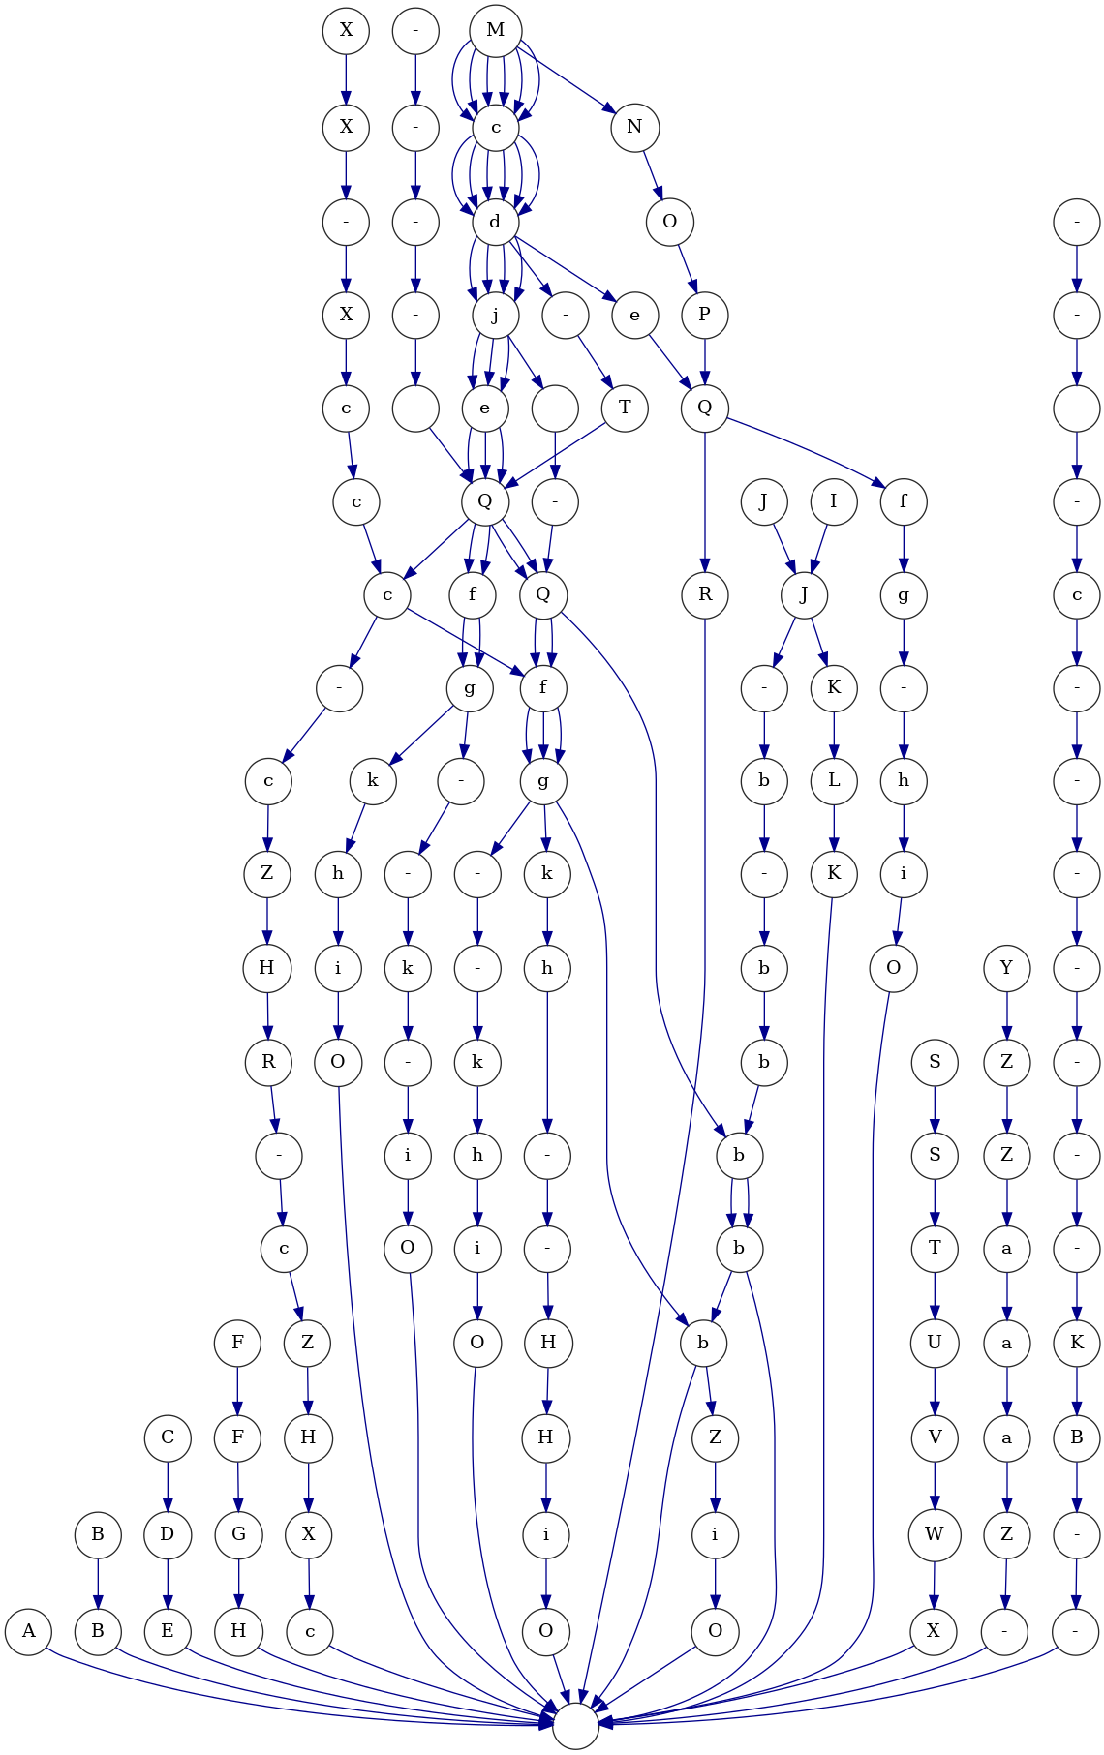
\includegraphics[width=0.8\linewidth]{Okamoto_fig/digraph-dtom.pdf}
        \vspace{-5mm}
	\caption{DtoMユーザの代表CTパスを可視化した状態遷移図}
	\label{fig:digraph-dtom}
\end{figure*}

\section{考察}

\subsection*{BtoDユーザ}

本分析は表\ref{tab:ranking-btod}に従い,BtoDユーザが習熟度向上の際に制作する作品のCTスコア重複数上位1件に属するユーザのみを抽出しているため,表\ref{tab:dict-btod}に示した本分析の対象ユーザが頻繁に獲得するCT概念が他ユーザのCTパスでも利用されるか調査した.結果として,表\ref{tab:dict-btod}の全てにおいて本分析の対象を除くユーザのCTパスでも各CT概念が最低873回以上獲得されていることが確認できた.したがって,本分析の結果は対象ユーザだけにとどまらず,全体のユーザに対しても当てはまることが示唆された.また,作品制作数を跨いで最多で出現したBのスキルについても本分析の対象を除くユーザのCTパスでの獲得回数を調査した.結果として,重複を含めて,1,966回獲得されていることが確認できた.BtoDユーザがCTスキルを獲得する回数の合計は20,558回であり,約10\%の確率でBtoDユーザはBのスキルを獲得することが示唆された.

\subsection*{DtoMユーザ}

本分析は表\ref{tab:ranking-dtom}に従い,DtoMユーザが習熟度向上の際に制作する作品のCTスコア重複数上位1件に属するユーザのみを抽出しているため,表\ref{tab:dict-dtom}に示した本分析の対象ユーザが頻繁に獲得するCT概念が他ユーザのCTパスでも利用されるかの調査をBtoDユーザ同様に行った.結果として,表\ref{tab:dict-dtom}の全てにおいて本分析の対象を除くユーザのCTパスでも各CT概念が最低23回以上獲得されていることが確認できた.したがって,本分析の結果は対象ユーザだけにとどまらず,全体のユーザに対しても当てはまることが示唆された.

\chapter{RQ2:ユーザが獲得してきたCT7概念から次の作品でCT習熟度が向上するかどうかを予測することは可能か?}
\section{CT習熟度到達タイミングの予測}
本章ではユーザのCT獲得過程に基づいて,ユーザが次に制作する作品が特定の習熟度以上の評価を得るかを予測するモデルとして,習熟度到達予測モデルを構築し,従来モデルとの比較を行う.また,評価結果を基に,モデルの精度に寄与する要因と従来モデルとの予測結果の特徴の違いについて考察する.
\section{分析手法}
\subsection{CT習熟度到達予測モデルの構築}
従来研究より,目的変数の異なる2種類の予測モデルを構築する.

\begin{description}
\item [BtoDモデル:]CTスコアが8点以上(Developing以上)のオリジナル作品を制作するユーザを予測
\item [DtoMモデル:]CTスコアが15以上(Master)のオリジナル作品を制作するユーザを予測
\end{description}

目的変数は,{$N~(3 \leq N \leq 20)$}番目にDeveloping以上またはMasterに到達するオリジナル作品を制作したユーザを正例クラス,それ以外のユーザを負例クラスとする.例えば,BtoDモデルの構築では2番目以降に制作するオリジナル作品でDeveloping以上の評価を得るユーザを正例クラスとし,そうでないユーザを負例クラスとして扱う.また従来研究~\cite{Ando_2021}では,ユーザが目標の習熟度を満たす作品を1回でも制作すれば当該習熟度に到達すると判断しているため,本研究でも同様に扱う.構築するモデルでは,ユーザがオリジナル作品で目標習熟度以上のCTスコア合計点を獲得した場合のみ到達したと判断し,リミックス作品によるCTスコア合計点の獲得は目標習熟度に到達したと判定しない.また,N=1となる正例クラスは,特徴量として説明する作品数が0件となるため,モデルの構築時には除外する.

\ref{sec:3-analysis}節の結果より,BtoDユーザとDtoMユーザが作品制作過程で獲得するCT概念には特徴があったことから,従来モデルで用いた説明変数と本節で提案するCTパス重複数を考慮した説明変数を結合してモデルを学習する.

従来モデルでは,説明変数としてユーザが過去20作品を制作する中で使用したCT7概念の点数(0点から3点の4種類)までの獲得有無を用いた.また,従来研究\cite{Dasgupta_2016}よりリミックス作品の制作による学習効果も示されていることから,オリジナル作品とリミックス作品で獲得した点数を区別している.したがって,本実験でも従来研究と同様に$7(7つのCT概念) \times 4(0点から3点) \times 2(オリジナル作品またはリミックス作品)$の計56次元の説明変数を計測する.さらに本研究ではユーザの作品制作過程を捉えるための新しい説明変数を提案する.

本実験ではモデルの学習時にユーザの作品制作過程を考慮するため,ユーザが目標習熟度に次の作品で到達する確率としてパス遷移確率$P$を計測する.

まず,対象ユーザ群から\ref{sec:chapter_3-2}節と同様に,各ノード間のCTパス重複数を算出する.
パス遷移確率$P_{n,m}$は,ユーザが$n$番目に制作する作品から$m$番目に制作する作品,つまりノード$n$からノード$m$番目に到達する確率を意味し,式\ref{formula: single-ct-path}と式\ref{formula:ct-path}から算出する.ここで$N+1=\{ {n + 1}_1, {n + 1}_2,\ldots,{n + 1}_{k-1}, {n + 1}_k  \}$は,$n$の次に遷移するノード$n+1$の全体集合を意味し,式\ref{formula:ct-path}の分母はノード$n$からN+1に遷移するCTパス重複数の合計数である.

\begin{equation}
  B_n = \frac{nからn+1のCT
  パス重複数}{\sum_{j=1}^{k} (nからn+1_jのCTパス重複数)} \label{formula: single-ct-path}
\end{equation}

% \begin{equation}
%   P_n = B_n \times P_{n-1} (P_1 = B_1) \label{formula:ct-path}
% \end{equation}

\begin{equation}\label{formula:ct-path}
  P_{n,m} = B_m \times B_{m-1} \times \ldots \times B_{n+1} \times P_n \quad 
\end{equation}

本実験ではユーザの作品制作過程をモデルに反映するため,ユーザが制作する$n$番目の作品から$m$番目までの各パス遷移確率の集合$P_{i,i+1}|(n \leq i \leq m - 1)=\{P_{n,n+1}, P_{n+1,n+2}, \dots, P_{m-2, m-1}, P_{m-1, m}\}$を全て計測する.また,作品$m$は対象ユーザ群のうち,各ユーザが最後に制作した作品のひとつ前の作品とし,$n-m$の作品間ノード数$L$がモデルに与える影響も調査するため,作品$n$には$\{m-1, m-2,\dots, m-(L-1), m-L\}$を順に代入し,$P_{i,i+1}|(n \leq i \leq m - 1)$を算出する.この時,対象ユーザの作品数がLに満たない場合,そのユーザはモデルの学習から除外することとする.

本実験には,\ref{sec:chapter_3-1}節で収集したユーザ6,323人が1番目から20番目までに制作した作品126,460件を使用する.提案モデルの説明変数の計測には,最低限ユーザが3作品制作している必要があるため,ユーザ6,323人の中で3作品以上20作品以内の制作数を持つユーザ3,810人を対象とする.したがって,
CT概念獲得有無と,パス遷移確率$P$を結合した計$56+L \mid (1 \leq L \leq 18)$次元の説明変数を計測し,$L\mid (1 \leq L \leq 18)$個のBtoDモデル,DtoMモデルを構築する.

本論文では,ユーザの作品制作過程に基づく習熟度到達予測モデルの構築にランダムフォレスト~\cite{Breiman_2001}を用いる.ランダムフォレストのパラメータは従来研究との比較を行うために,作成する決定木の個数は200個,各決定木の作成に使用する特徴量の個数は各モデルの説明変数が持つ次元の平方根とする.また,クラス間の偏りを解消するため,モデル構築時に各クラスに出現する割合の逆数に基づいた重みづけを行う.例えば,対象ユーザが300人中,正例クラスが20人,負例クラスが280であった場合,それぞれのクラスの事例に300 / 20 = 15,300 / 280 = 1.07の重みを割り当てる.

予測モデルの評価指標には適合率,再現率,F値を使用する.本研究では,交差検証によって10回の予測モデルの構築を行い,それぞれの予測結果で得られた3つの評価指標の平均値を算出し,評価を行う.また,本実験では,10個の各予測モデルから得られる説明変数の順位を分類し,本実験で提案する説明変数の分類精度への影響度を確認する.

\section{実験結果}

本節では,2つの習熟度到達予測モデル(BtoDモデル,DtoMモデル)のうち,説明変数として与えるパスの長さ$L$毎の精度評価と,従来モデルとの精度比較,および分類精度に寄与する説明変数について述べる.

\subsection{モデルの分類精度}\label{subsec:model-result}

\begin{figure*}[t]
	\centering
	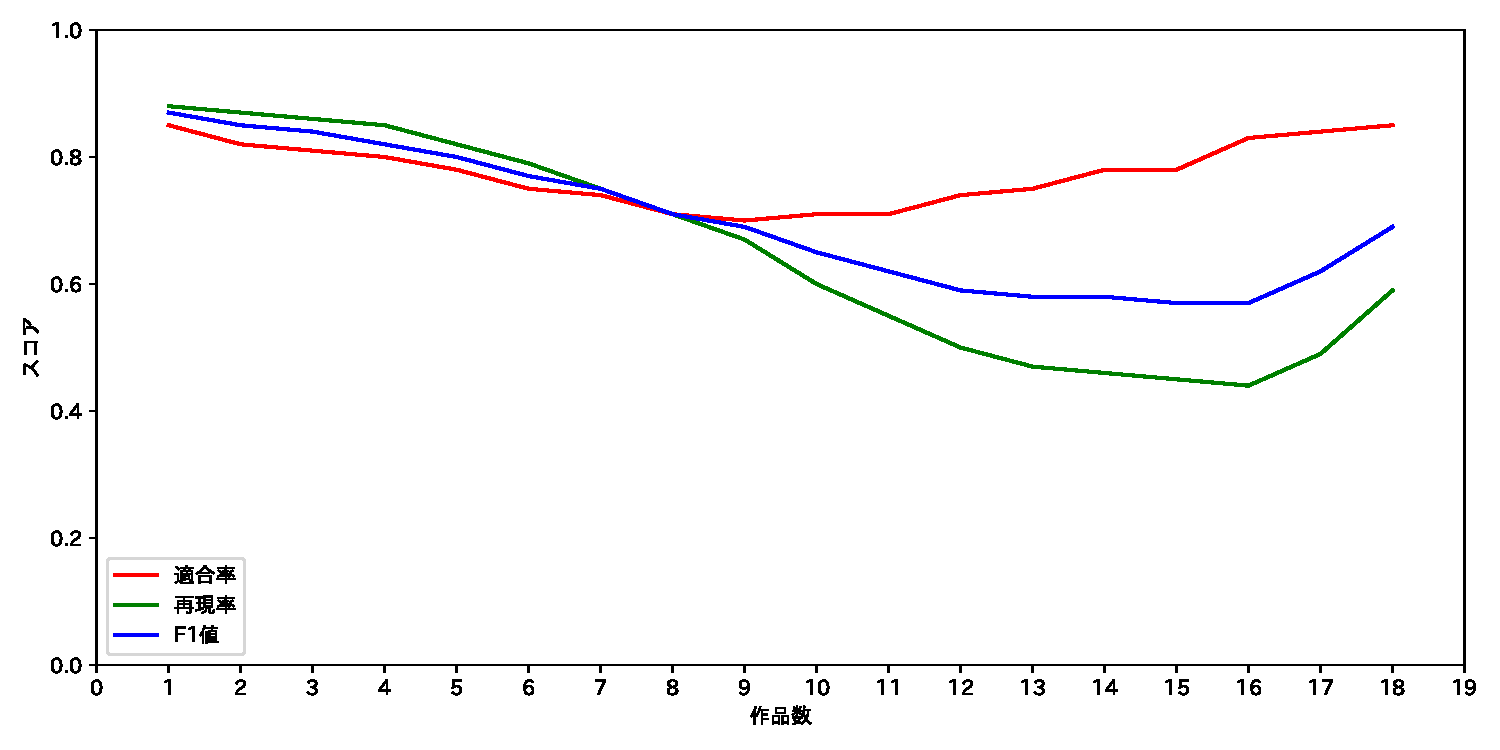
\includegraphics[width=1.0\linewidth]{Okamoto_fig/btod-lines2.pdf}
	\caption{提案BtoDモデルの作品数ごとの評価指標の遷移}
	\label{fig:btod-lines}
\end{figure*}

\begin{table}
  \caption{従来BtoDモデルと提案BtoDモデル(L=1)の精度比較}
  \label{tab:btod-model-comp}
  \vspace{2mm}
  \centering
  \begin{tabular}{l|c|c|c|c|c}
    \hline
     & 適合率 & 再現率 & F1値 & \begin{tabular}[c]{@{}c@{}}正確に予測できた\\BtoDユーザ数\end{tabular} & \begin{tabular}[c]{@{}c@{}}誤って予測された\\BtoDユーザ数\end{tabular}\\
    \hline
    \hline
    従来BtoDモデル & 0.84 & 0.86 & 0.85 & 2,333 & 370\\
    \hline
    提案BtoDモデル(L=1) & \textbf{0.85} & \textbf{0.88} & \textbf{0.87}  & 2,388 & 315\\
    \hline
  \end{tabular}
\end{table}


図\ref{fig:btod-lines}は,構築したBtoDモデルにおいて作品間ノード数$L$ごとの分類精度(適合率,再現率,F値)を示す.縦軸は評価スコア,横軸は作品間ノード数$L$を意味する.各分類精度は,層化10分割交差検証により出力した10回分の精度の平均値を表している.BtoDモデルの評価指標はノード数$L=1$のときに最も高い数値となり,適合率は0.85,再現率は0.88,F値は0.87であった.表\ref{tab:btod-model-comp}は従来BtoDモデルと提案BtoDモデルのうち,最も精度の高かったノード数$L=1$の分類精度と正しく予測されたBtoDユーザ数,誤って非BtoDユーザであると予測されたBtoDユーザ数を示す.従来BtoDモデルではDeveloping以上に到達したユーザに対して正しく予測できた数が2,333であるのに対し,提案BtoDモデルでは2,388であることから,提案BtoDモデルによって55人の習熟度向上ユーザが正しく予測できるようになったといえる.また,従来BtoDモデルではDeveloping以上に到達したユーザに対して到達していないと誤分類されたユーザ数が370であるのに対し,提案BtoDモデルでは315であることから,提案BtoDモデルによって55人のDeveloping以上に到達したユーザに対して誤分類が減ったといえる.従来BtoDモデルの適合率は0.84,再現率は0.86,F1値は0.85であり,提案BtoDモデルの適合率は0.85,再現率は0.88,F1値は0.87であることから,提案BtoDモデルは従来BtoDモデルと比べて適合率,再現率,F値において上回っているため,Developingに到達するユーザは直近に同じCT概念を持つ作品を制作することが多く,一度もDevelopingに到達しなかったユーザは直近に異なるCT概念を持つ作品を制作することが多いことが示唆される.

図\ref{fig:dtom-lines}は,構築したDtoMモデルにおいて作品間ノード数$L$ごとの分類精度(適合率,再現率,F値)を示す.縦軸は評価スコア,横軸は作品間ノード数$L$を意味する.各分類精度は,層化10分割交差検証により出力した10回分の精度の平均値を表している.BtoDモデルの適合率はノード数$L=9$のときに最も高い0.80となり,再現率,F値はノード数$L=1$のときに最も高くなり,それぞれ0.43,0.55であった.表\ref{tab:dtom-model-comp}は従来DtoMモデルと提案DtoMモデルのうち,最もF値が高かったノード数$L=1$の分類精度と習熟度が向上したと予測された非BtoDユーザ数を示す.従来DtoMモデルではMaster以上に到達したユーザに対して到達していないと誤分類されたユーザ数が207であるのに対し,提案DtoMモデルでは144であることから,提案DtoMモデルによって63人のMasterに到達しなかったユーザに対して誤分類が減ったといえる.従来DtoMモデルの適合率は0.70,再現率は0.44,F1値は0.54であり,提案DtoMモデルの適合率は0.77,再現率は0.45,F1値は0.59であった.従来DtoMモデルと比べて提案DtoMモデルは適合率,F値において上回っているため,BtoDモデルと同様に,Masterに到達するユーザは直近に同じCT概念を持つ作品を制作することが多く,一度もMasterに到達しなかったユーザは直近に異なるCT概念を持つ作品を制作することが多いことが示唆される.

\begin{figure*}[t]
	\centering
	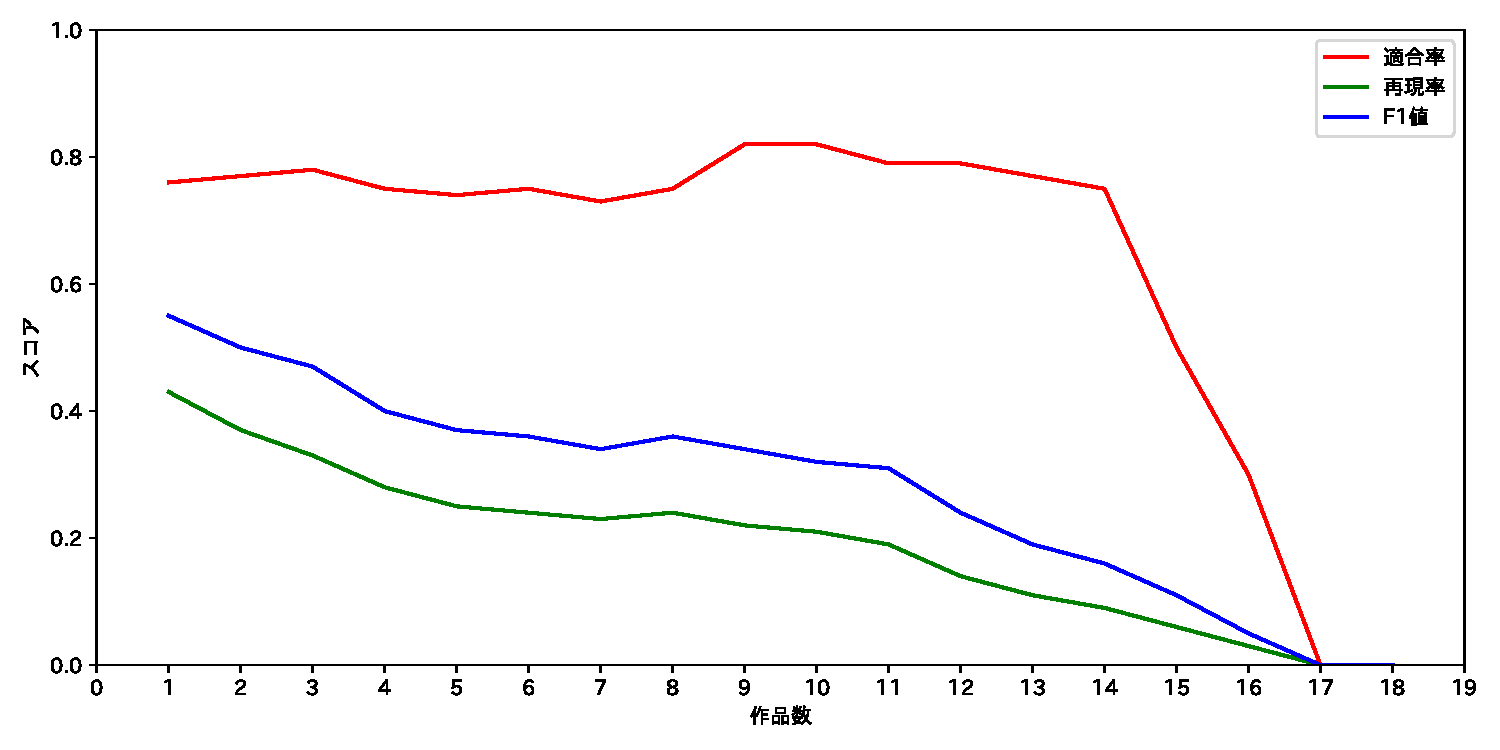
\includegraphics[width=1.0\linewidth]{Okamoto_fig/dtom-lines2.pdf}
	\caption{提案DtoMモデルの作品数ごとの評価指標の遷移}
	\label{fig:dtom-lines}
\end{figure*}

\begin{table}
  \caption{従来DtoMモデルと提案DtoMモデル(L=1)の精度比較}
  \label{tab:dtom-model-comp}
  \vspace{2mm}
  \centering
  \begin{tabular}{l|c|c|c|c}
    \hline
     & 適合率 & 再現率 & F1値 & \begin{tabular}[c]{@{}c@{}}誤って予測された\\非BtoDユーザ数\end{tabular}\\
    \hline
    \hline
    従来DtoMモデル & 0.70 & \textbf{0.44} & 0.54 & 207 \\
    \hline
    提案DtoMモデル(L=1) & \textbf{0.79} & \textbf{0.44} & \textbf{0.57} & 144 \\
    \hline
  \end{tabular}
\end{table}

\subsection{特徴量重要度}\label{subsec:importance}

\begin{table}[t]
    \caption{従来BtoDモデルと提案BtoDモデル(L=1)における重要度の高い説明変数の上位10件}\label{tab:feature_importance-btod}
    \centering
    \scalebox{0.85}{
        \begin{tabular}{r|rp{60mm}|rp{60mm}}
            \hline
            & \multicolumn{2}{c|}{従来BtoDモデル} & \multicolumn{2}{c}{提案BtoDモデル(L=1)} \\ \cline{2-5}
            グループ & \begin{tabular}{r} 重要度 \end{tabular} & \begin{tabular}{c} 説明変数 \end{tabular} & \begin{tabular}{r} 重要度 \end{tabular} & \begin{tabular}{c} 説明変数 \end{tabular} \\ \hline \hline
            1 & \begin{tabular}{r}0.05\end{tabular} & \begin{tabular}{r} \{オリジナル/フロー制御/0点\} \end{tabular} & \begin{tabular}{r} 0.20 \end{tabular} & \begin{tabular}{l} \{パス遷移確率P_{m-1,m} \} \end{tabular} \\ \hline
            2 & \begin{tabular}{r} 0.04 \end{tabular} & \begin{tabular}{r} \{リミックス/抽象化/0点\} \end{tabular} & \begin{tabular}{r} 0.04 \end{tabular} & \begin{tabular}{l} \{リミックス/データ表現/0点\} \end{tabular} \\ \hline
            3 & \begin{tabular}{r} 0.04 \end{tabular} & \begin{tabular}{r} \{オリジナル/データ表現/0点\} \end{tabular} & \begin{tabular}{r} 0.03 \end{tabular} & \begin{tabular}{l} \{オリジナル/ユーザ対話性/0点\} \end{tabular} \\ \hline
            4 & \begin{tabular}{r} 0.04 \end{tabular} & \begin{tabular}{r} \{オリジナル/ユーザ対話性/0点\} \end{tabular} & \begin{tabular}{r} 0.03 \end{tabular} & \begin{tabular}{l} \{オリジナル/フロー制御/0点\} \end{tabular} \\ \hline
            5 & \begin{tabular}{r} 0.04 \end{tabular} & \begin{tabular}{r} \{リミックス/並列/0点\} \end{tabular} & \begin{tabular}{r} 0.03 \end{tabular} & \begin{tabular}{l} \{リミックス/抽象化/2点\} \end{tabular} \\ \hline
            6 & \begin{tabular}{r} 0.04 \end{tabular} & \begin{tabular}{r} \{リミックス/データ表現/0点\} \end{tabular} & \begin{tabular}{r} 0.03 \end{tabular} & \begin{tabular}{l} \{リミックス/並列/0点\} \end{tabular} \\ \hline
            7 & \begin{tabular}{r} 0.04 \end{tabular} & \begin{tabular}{r} \{リミックス/抽象化/2点\} \end{tabular} & \begin{tabular}{r} 0.03 \end{tabular} & \begin{tabular}{l} \{オリジナル/データ表現/0点\} \end{tabular} \\ \hline
            8 & \begin{tabular}{r} 0.03 \end{tabular} & \begin{tabular}{r} \{リミックス/同期/0点\} \end{tabular} & \begin{tabular}{r} 0.03 \end{tabular} & \begin{tabular}{l} \{リミックス/抽象化/0点\} \end{tabular} \\ \hline
            9 & \begin{tabular}{r} 0.03 \end{tabular} & \begin{tabular}{r} \{リミックス/フロー制御/1点\} \end{tabular} & \begin{tabular}{r} 0.03 \end{tabular} & \begin{tabular}{l} \{リミックス/同期/0点\} \end{tabular} \\ \hline
            10 & \begin{tabular}{r} 0.03 \end{tabular} & \begin{tabular}{r} \{リミックス/論理/3点\} \end{tabular} & \begin{tabular}{r} 0.03 \end{tabular} & \begin{tabular}{l} \{リミックス/フロー制御/1点\} \end{tabular} \\ \hline
        \end{tabular}
    }
    \vspace{3mm}
\end{table}

\begin{table}[t]
    \caption{従来DtoMモデルと提案DtoMモデル(L=1)における重要度の高い説明変数の上位10件}\label{tab:feature_importance-dtom}
    \centering
    \scalebox{0.85}{
        \begin{tabular}{r|rp{60mm}|rp{60mm}}
            \hline
            & \multicolumn{2}{c|}{従来DtoMモデル} & \multicolumn{2}{c}{提案DtoMモデル(L=1)} \\ \cline{2-5}
            グループ & \begin{tabular}{r} 重要度 \end{tabular} & \begin{tabular}{c} 説明変数 \end{tabular} & \begin{tabular}{r} 重要度 \end{tabular} & \begin{tabular}{c} 説明変数 \end{tabular} \\ \hline \hline
            1 & \begin{tabular}{r} 0.04 \end{tabular} & \begin{tabular}{l} \{オリジナル/データ表現/0点\} \end{tabular} & \begin{tabular}{r} 0.12 \end{tabular} & \begin{tabular}{l} \{パス遷移確率P_{m-1,m}\} \end{tabular} \\ \hline
            2 & \begin{tabular}{r} 0.04 \end{tabular} & \begin{tabular}{r} \{オリジナル/抽象化/0点\} \end{tabular} & \begin{tabular}{r} 0.05 \end{tabular} & \begin{tabular}{l} \{オリジナル/同期/2点\} \end{tabular} \\ \hline
            3 & \begin{tabular}{r} 0.03 \end{tabular} & \begin{tabular}{r} \{オリジナル/同期/2点\} \end{tabular} & \begin{tabular}{r} 0.04 \end{tabular} & \begin{tabular}{l} \{オリジナル/抽象化/0点\} \end{tabular} \\ \hline
            4 & \begin{tabular}{r} 0.03 \end{tabular} & \begin{tabular}{r} \{オリジナル/フロー制御/3点\} \end{tabular} & \begin{tabular}{r} 0.03 \end{tabular} & \begin{tabular}{l} \{オリジナル/データ表現/0点\} \end{tabular} \\ \hline
            5 & \begin{tabular}{r} 0.03 \end{tabular} & \begin{tabular}{r} \{リミックス/同期/0点\} \end{tabular} & \begin{tabular}{r} 0.03 \end{tabular} & \begin{tabular}{l} \{リミックス/同期/0点\} \end{tabular} \\ \hline
            6 & \begin{tabular}{r} 0.03 \end{tabular} & \begin{tabular}{l} \{オリジナル/論理/0点\} \\ \{オリジナル/フロー制御/1点\} \\ \{リミックス/論理/0点\} \end{tabular} & \begin{tabular}{r} 0.03 \end{tabular} & \begin{tabular}{l} \{オリジナル/フロー制御/3点\} \end{tabular} \\ \hline
            7 & \begin{tabular}{r} 0.03 \end{tabular} & \begin{tabular}{r} \{オリジナル/並列/3点\} \end{tabular} & \begin{tabular}{r} 0.03 \end{tabular} & \begin{tabular}{l} \{オリジナル/並列/3点\} \end{tabular} \\ \hline
            8 & \begin{tabular}{r} 0.03 \end{tabular} & \begin{tabular}{r} \{オリジナル/同期/3点\} \end{tabular} & \begin{tabular}{r} 0.03 \end{tabular} & \begin{tabular}{l} \{オリジナル/データ表現/2点\} \end{tabular} \\ \hline
            9 & \begin{tabular}{r} 0.03 \end{tabular} & \begin{tabular}{r} \{リミックス/フロー制御/1点\} \end{tabular} & \begin{tabular}{r} 0.03 \end{tabular} & \begin{tabular}{l} \{オリジナル/並列/2点\} \\ \{リミックス/並列/0点\} \end{tabular} \\ \hline
            10 & \begin{tabular}{r} 0.03 \end{tabular} & \begin{tabular}{r} \{オリジナル/論理/2点\} \end{tabular} & \begin{tabular}{r} 0.03 \end{tabular} & \begin{tabular}{l} \{オリジナル/同期/3点\} \end{tabular} \\ \hline
        \end{tabular}
    }
    \vspace{3mm}
\end{table}

表\ref{tab:feature_importance-btod}と表\ref{tab:feature_importance-dtom}はそれぞれ従来BtoDモデルと提案BtoDモデル,従来DtoMモデルと提案DtoMモデルにおいて,分類精度に寄与した説明変数を重要度の高いグループ順に並び替えた結果を示す.重要度の値は,層化10分割交差検証により出力した10回分の重要度の平均値を示す.また,分類精度に寄与する説明変数はCT概念の場合,\{作品の種類/CT概念,点数\}のように示す.

表\ref{tab:feature_importance-btod}より,従来BtoDモデルでは,説明変数\{オリジナル/フロー制御/0点\}が分類精度に最も寄与し,続いて\{リミックス/抽象化/0点\},\{オリジナル/データ表現/0点\}が寄与しているのに対し,提案BtoDモデルでは本実験で提案した説明変数\{遷移確率$P_{m-1,m}$\}が分類精度に最も寄与し,続いて\{リミックス/データ表現/0点\},\{オリジナル/ユーザ対話性/0点\}が寄与していることがわかった.

表\ref{tab:feature_importance-dtom}より,従来DtoMモデルでは,説明変数\{オリジナル/データ表現/0点\}が分類精度に最も寄与し,続いて\{オリジナル/抽象化/0点\},\{オリジナル/同期/2点\}が寄与しているのに対し,提案BtoDモデルでは本実験で提案した説明変数\{遷移確率$P_{m-1,m}$\}が分類精度に最も寄与し,続いて\{オリジナル/同期/2点\},\{オリジナル/抽象化/0点\}が寄与していることがわかった.

従来BtoDモデルと従来DtoMモデルにおいて最も分類精度に寄与した説明変数と次に重要度の大きい説明変数との重要度の差はどちらも0.01程度であったが,提案BtoDモデルにおいて最も分類精度に寄与した\{遷移確率$P_{m-1,m}$\}の重要度は次に大きい\{リミックス/データ表現/0点\}の重要度の約5倍,また提案BtoDモデルにおいて最も分類精度に寄与した\{遷移確率$P_{m-1,m}$\}の重要度は次に大きい\{オリジナル/同期/2点\}の重要度の約2.4倍であることから,本提案モデルで用いた説明変数は予測に対して有効に働き,重要な指標であることが示唆される.


\section{考察}

本節では,構築した習熟度到達予測を行う従来モデルと提案モデルの評価結果に基づき,提案モデルの精度に起因する要因と,従来モデル,提案モデルで予測できた作品と予測できなかった作品とその特徴について考察する.

\subsection{提案モデルの精度に起因する要因}

\ref{subsec:model-result}節に示された通り,2種類の提案モデルに学習させる遷移確率$P$が1つの時に最高の精度を達成し,\ref{subsec:importance}節では,遷移確率$P$の特徴量重要度が高かったことから,特定の習熟度に到達するユーザと到達しないユーザ間では,作品M−1から作品Mへの遷移確率に差があることが示唆された.

図\ref{fig:add-btod}はDevelopingの習熟度に到達したユーザ(BtoDユーザ)とDevelopingに到達しなかったユーザ(非BtoDユーザ)が直前の作品に遷移する際のパスの重複数の分布を比較している.BtoDユーザの中央値は7.0,非BtoDユーザの中央値は3.0であり,Man-whitney U検定を実施したところ,統計的に有意な差(p$<$0.05)が確認できた.これは,Developingの習熟度に到達するユーザが頻繁に通るパスを辿るのに対し,到達しないユーザはあまり再現性のないパスを通っていることが示唆された.

また,図\ref{fig:add-dtom}はMasterの習熟度に到達したユーザ(DtoMユーザ)と,Developingに到達しなかったユーザ(非BtoDユーザ)が直前の作品に遷移する際のパスの重複数の分布を示す.DtoMユーザの中央値は2.0,非DtoMユーザの中央値は4.0であり,Man-whitney U検定を実施したところ,統計的に有意な差(p$<$0.05)を確認できた.Masterの習熟度に到達するユーザがより多様な作品から遷移する傾向にあること,また到達しないユーザはより再現性のあるパスを辿る傾向にあることを示している.


\begin{figure*}[t]
	\centering
	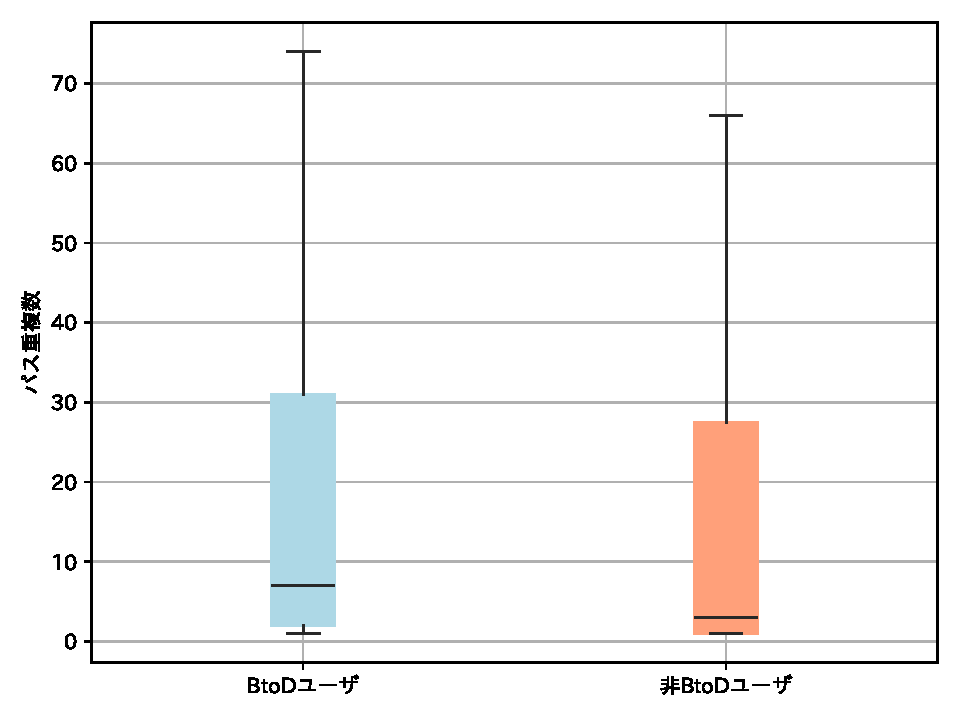
\includegraphics[width=0.7\linewidth]{Okamoto_fig/add-btod.pdf}
	\caption{BtoDユーザが直前の作品を制作する前のCTパス重複数}
	\label{fig:add-btod}
\end{figure*}

\begin{figure*}[t]
	\centering
	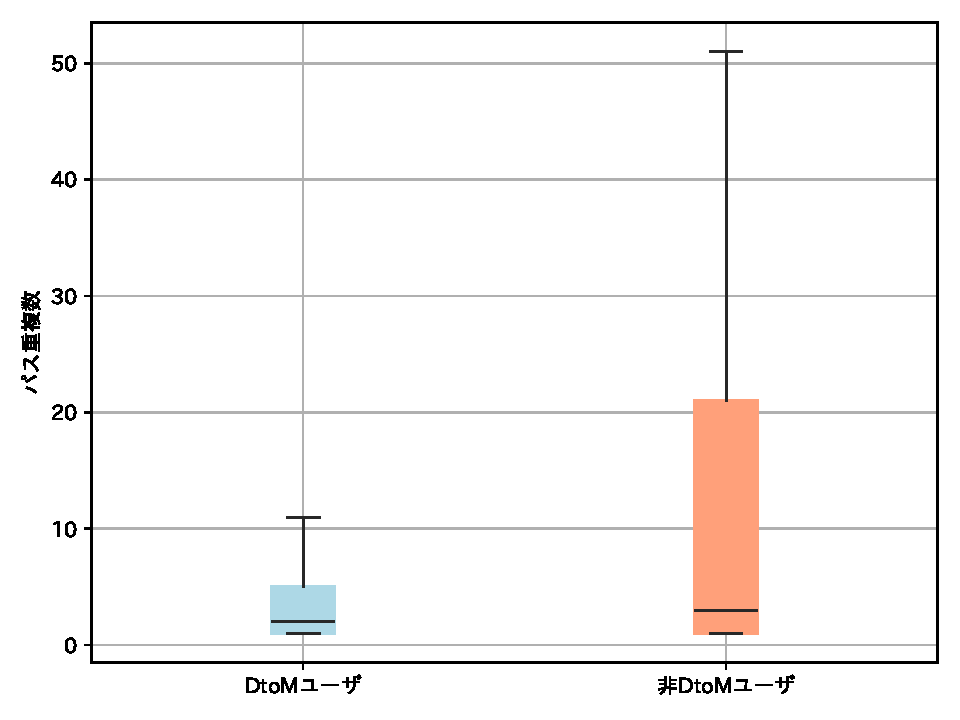
\includegraphics[width=0.7\linewidth]{Okamoto_fig/add-dtom.pdf}
	\caption{DtoMユーザが直前の作品を制作する前のCTパス重複数}
	\label{fig:add-dtom}
\end{figure*}



\subsection{従来モデルと提案モデルで予測できたユーザと予測できなかったユーザの特徴分析}

\subsubsection*{BtoDモデル}

図\ref{fig:btod-venn}に,従来BtoDモデルと提案BtoDモデルがそれぞれ予測できたユーザの数,両モデルが共に予測できたユーザの数,および予測できなかったユーザの数を示す.提案BtoDモデルでは,CTパスが同一で予測結果も一致したユーザのペアが12組見つかったが,従来BtoDモデルのみで予測できたユーザ内にはペアは見つからなかったことから,提案BtoDモデルによって作品制作過程を考慮した習熟度の到達予測が可能にしたことが示唆された.また,従来BtoDモデルと提案BtoDモデルで予測できたユーザは作品制作数の中央値が9.0であるのに対し,どちらのモデルでも予測できなかったユーザの作品制作数の中央値は19.0であった.Man-whitney U検定を実施したところ,統計的な有意差(p値$<$0.05)が確認できたことから,従来BtoDモデルと提案BtoDモデルでは作品制作数の多いユーザの作品制作過程は十分に考慮できておらず,分類が困難であることが示された.

\subsubsection*{DtoMモデル}

図\ref{fig:dtom-venn}に,従来DtoMモデルと提案DtoMモデルがそれぞれ予測できたユーザの数,両モデルが共に予測できたユーザの数,および予測できなかったユーザの数を示す.提案DtoMモデルで予測できたユーザの中でCTパスが同一で,予測結果が一致したユーザのペアは見つからなかった.このことから,\ref{sec:3-analysis}節で明らかにされた通り,DtoMユーザが多様なCTパスを通る傾向にあることを踏まえると,提案DtoMモデルでは作品制作過程を十分に考慮できていないことが示唆された.また,従来DtoMモデルと提案DtoMモデルで予測できたユーザは制作した作品数の中央値が17.0であるのに対し,どちらのモデルでも予測できなかったユーザが制作した作品数の中央値は11.0であった.Man-whitney U検定を実施したところ,統計的な有意差(p値$<$0.05)が確認できた.\ref{sec:3-analysis}節での分析により,DtoMユーザのうち,作品制作数が比較的少ないDtoMユーザの方がより多様性のあるCTパスを通る傾向にあることが明らかとなったことから,従来DtoMモデルと提案DtoMモデルでは作品制作数の比較的少ないユーザの作品制作過程は十分に考慮できていないことが示された.

\begin{figure*}[t]
	\centering
	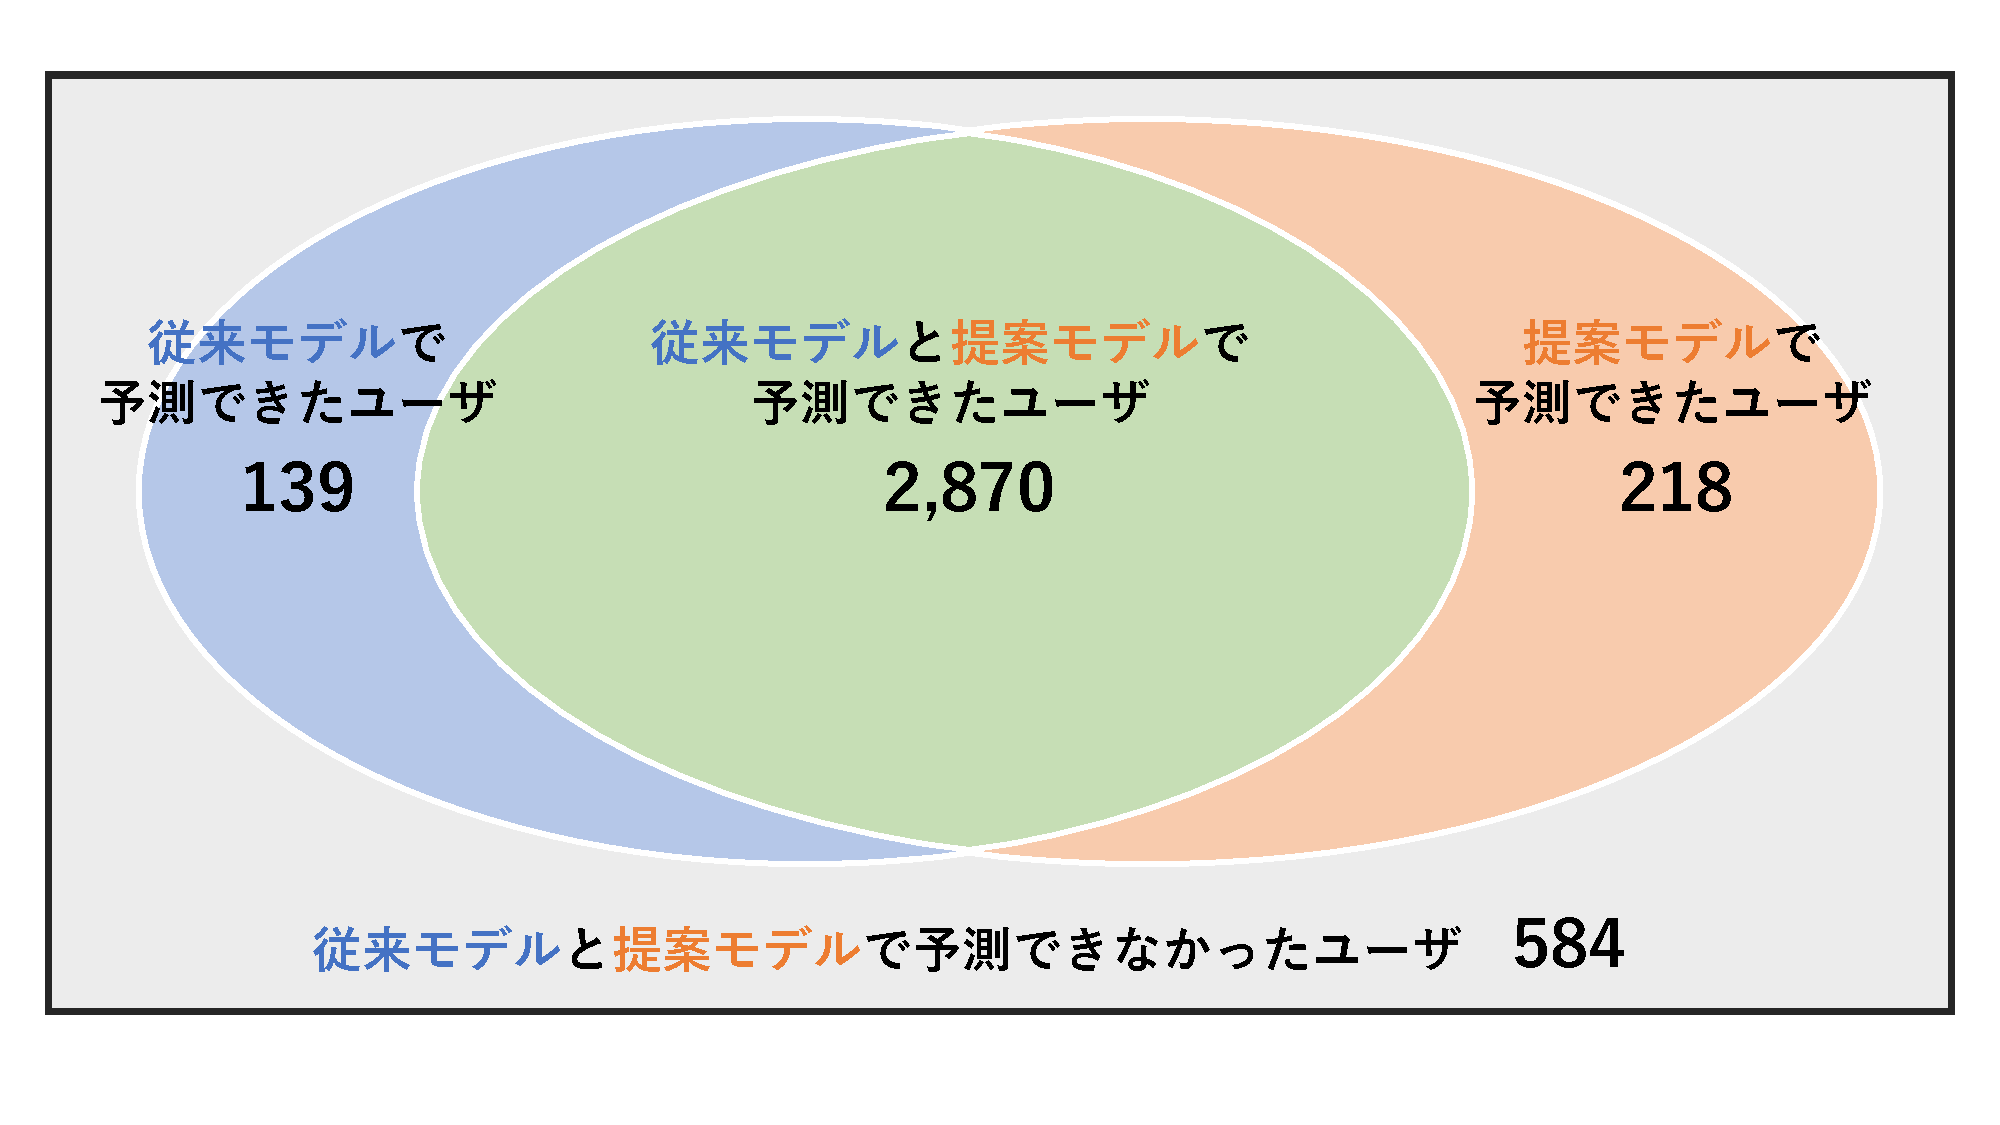
\includegraphics[width=1.0\linewidth]{Okamoto_fig/btod-venn.pdf}
        \vspace{-15mm}
	\caption{従来BtoDモデルと提案BtoDモデルで予測できたユーザと予測できなかったユーザ}
	\label{fig:btod-venn}
\end{figure*}

\begin{figure*}[t]
	\centering
	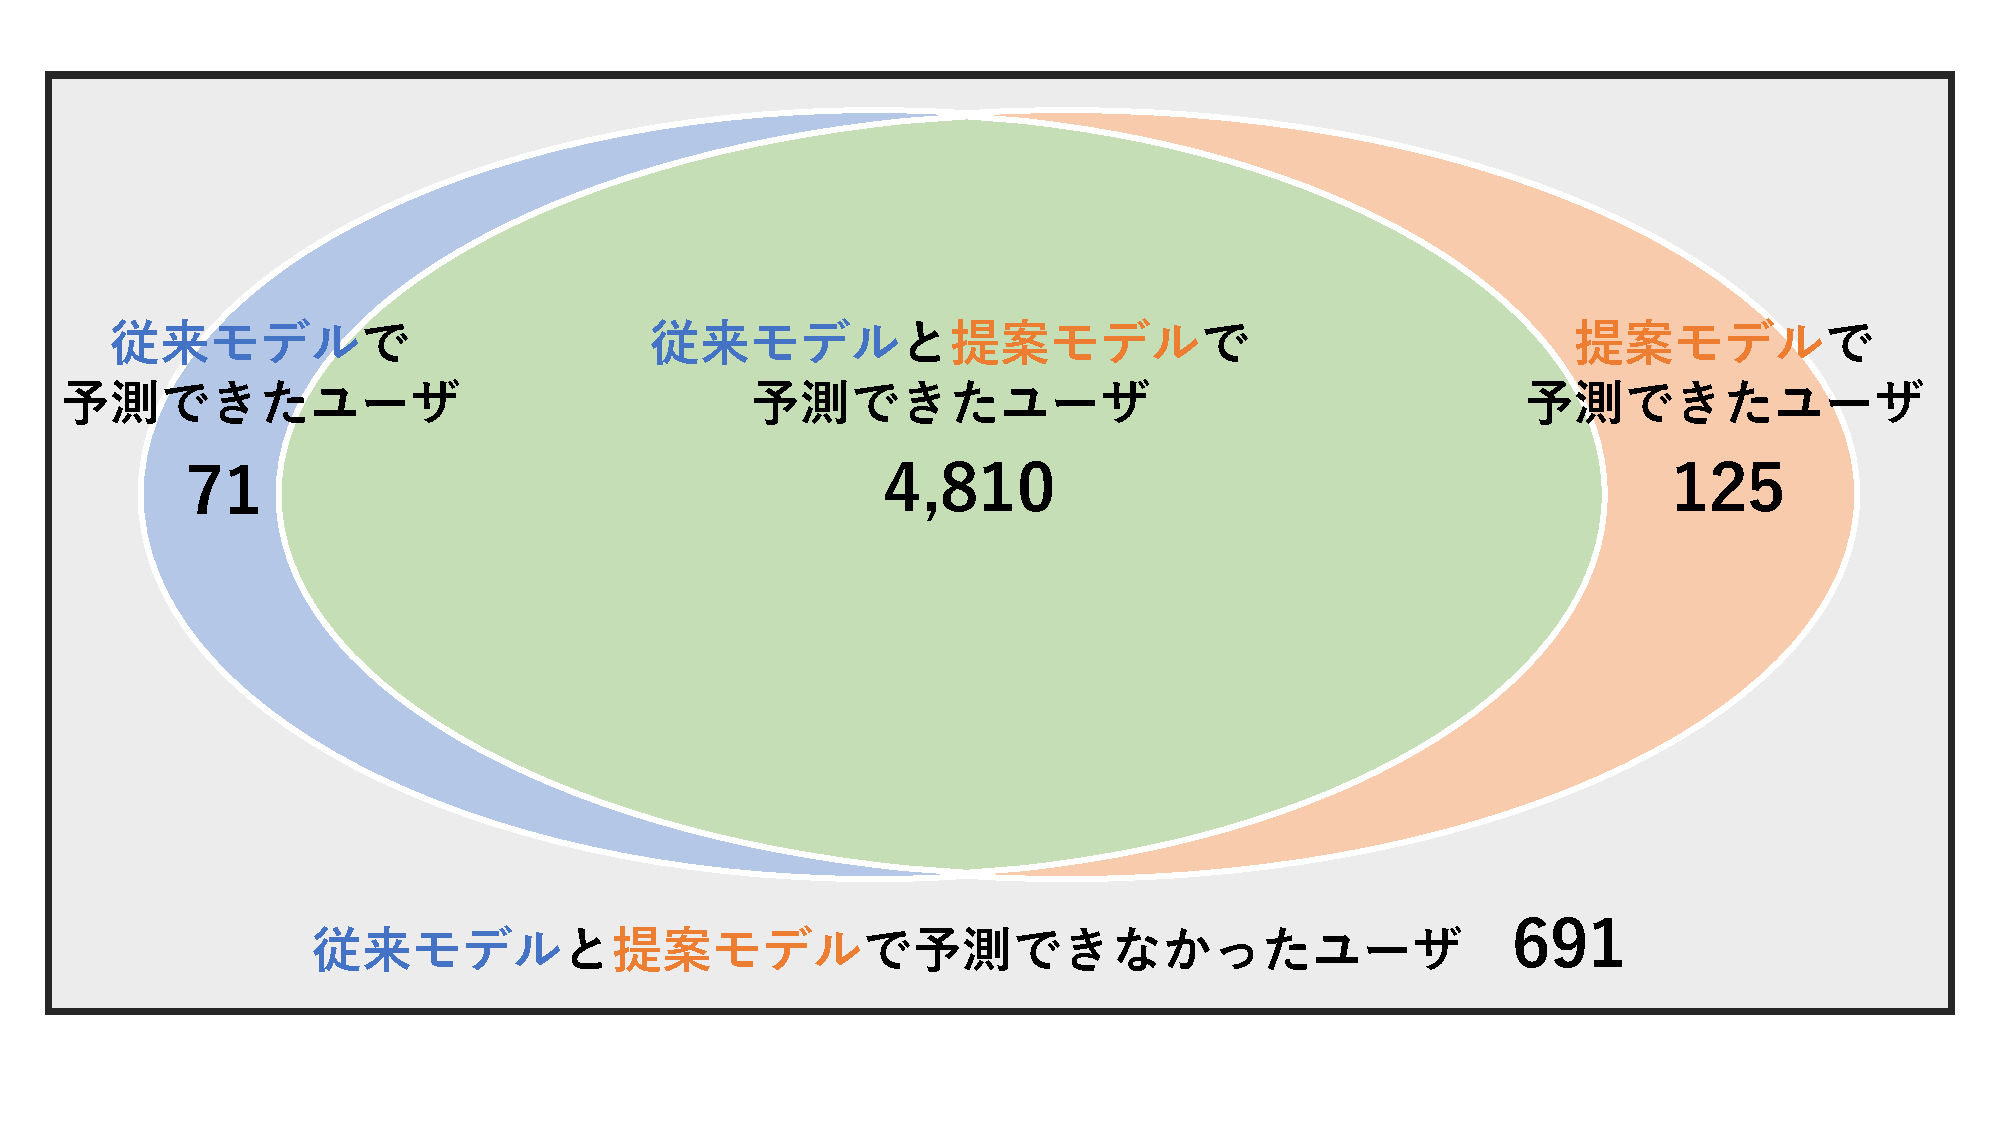
\includegraphics[width=1.0\linewidth]{Okamoto_fig/dtom-venn.pdf}
        \vspace{-15mm}
	\caption{従来DtoMモデルと提案DtoMモデルで予測できたユーザと予測できなかったユーザ}
	\label{fig:dtom-venn}
\end{figure*}



\chapter{妥当性への脅威}
\section{内的妥当性}

本論文では,ノード間の重複数をユーザの作品制作過程内の作品の重要な指標として捉えている.実際には,ユーザの作品制作過程の重要性を示す他の要因も存在することが考えられる.しかし,自由な作品制作環境下で,多くのユーザが複数回獲得されるCTスキルは作品制作過程において一定の重要性を持つと考える.

本論文では,ランダムフォレスト法を用いて習熟度到達予測モデルを構築した.構築した2つのモデルでは,正例クラスと負例クラスの数に偏りが存在したため,モデルの構築時に重みづけを行った.しかし,不均衡データの対応方法によってはモデルの予測精度に影響を与えることが考えられる.本論文では,層化10分割交差検証により,10個のモデルを構築した予測結果を用いることでその脅威を軽減する.

\section{外的妥当性}

本論文では,ユーザが実際にScratch上に公開する作品を基に習熟度到達予測モデルを構築した.その際にオリジナル作品の判断はScratch APIを用いて取得して情報を用いて行ったが,ユーザが他のユーザが制作した作品を模倣して制作する,あるいは他者に支援してもらい制作した作品が存在することも考えられる.これらの事例が対象ユーザに含まれている場合,分析結果やモデルの予測精度に違いが生じることが考えられるが,本論文ではユーザ6,323人が制作した作品126,460件を収集して多くの作品データを分析対象とすることで脅威を軽減する.




\chapter{おわりに}

本研究では,Scratchにおけるユーザのコンピュテーショナル・シンキング(CT)の作品制作過程に合わせた学習支援に向けて,まずユーザの作品制作過程の特徴を把握するために,ユーザが獲得してきたCT7概念の特徴量を分析した.分析の結果,BasicからDeveloping以上に到達するユーザの多くは同じCT概念の作品を繰り返し制作することが多く,共通して制作する作品があることがわかった.また,DevelopingからMasterに到達する多くのユーザは多様な作品を制作するものの,習熟度向上までに制作する作品数が多いユーザは共通したCT概念を持つ作品を制作することが多いことが明らかとなった.これらの分析結果を基に,ユーザの作品制作を考慮した説明変数を提案し,ユーザが次に特定の習熟度への到達するか否かを予測するモデルを構築して従来モデルとの比較を行った.結果として,提案モデルは従来モデルよりも精度が向上し,提案した説明変数がモデルの分類精度に最も影響を与えていることが明らかとなった.本研究により,ScratchにおけるユーザのCTスキル獲得状況に合わせた作品推薦等の学習支援の役立てとなることを期待する.
\|\end{document}|


%4.1
\subsection{表題・著者名等}

表題,著者名とその所属,および概要を前述のコマンドや環境により{\bf 和文と
英文の双方について}定義した後,\|\maketitle| によって出力する.


\newpage%%%%%

%4.1.1
\subsubsection{表題} 

表題は,\|\title| および \|\etitle| で定義した表題はセンタリングされる.
文字数の多いものについては,適宜 \|\\| を挿入して改行する.

%4.1.2
\subsubsection{著者名・所属} 

各著者の所属を第一著者から順に \|\affiliate| を用いてラベル(第1引数)を付けながら定義すると,
脚注に番号を付けて所属が出力される.
なお,複数の著者が同じ所属である場合には,
一度定義するだけで良い.



現在の所属は \|\paffiliate| を用い,同様にラベル,所属先を記述する.
所属先には自動で「現在」,
\|\\|の改行で「Presently with」が挿入される.
著者名は \|\author| で定義する.各著者名の直後に,英文著者名,
所属ラベルとメールアドレスを記入する.
著者が複数の場合は \|\author| を繰り返すことで,
2人,3人,\dots と増えていく.
現在の所属や,複数の所属先を追加する場合には,所属ラベルをカンマで区切り,追加すればよい.


また,メールアドレス部分は省略が可能である.





%4.1.3
\subsubsection{概要} 

和文の概要は \|abstract| 環境の中に,
英文の概要は \|eabstract| 環境の中に,それぞれ記述する.



%4.2
\subsection{本文}

%4.2.1
\subsubsection{見出し}

節や小節の見出しには \|\section|, \|\subsection|, \|\subsubsection|,
\|\paragraph| といったコマンドを使用する.

\<「定義」,「定理」などについては,\|\newtheorem|で適宜環境を宣言し,そ
の環境を用いて記述する.

%4.2.2
\subsubsection{行送り}

2段組を採用しており,左右の段で行の基準線の位置が一致することを原則としている.
また,節見出しなど,
行の間隔を他よりたくさんとった方が読みやすい場所では,
この原則を守るようにスタイルファイルが自動的にスペースを挿入する.
したがって本文中では \|\vspace| や \|\vskip| を用いたスペースの調整を行なわないようにすること.


%4.2.3
\subsubsection{フォントサイズ}

フォントサイズは,スタイルファイルによって自動的に設定されるため,
基本的には著者が自分でフォントサイズを変更する必要はない.

%4.2.4
\subsubsection{句読点}

句点には全角の「.」,
読点には全角の「,」を用いる.
ただし英文中や数式中で「.」や「,」を使う場合には,
半角文字を使う.「。」や「、」は使わない.



%4.2.5
\subsubsection{全角文字と半角文字}

全角文字と半角文字の両方にある文字は次のように使い分ける.

\begin{enumerate}
\item 括弧は全角の「(」と「)」を用いる.但し,英文の概要,図表見出し,
書誌データでは半角の「(」と「)」を用いる.

\item 英数字,空白,記号類は半角文字を用いる.ただし,句読点に関しては,
前項で述べたような例外がある.

\item カタカナは全角文字を用いる.

\item 引用符では開きと閉じを区別する.
開きには \|``| を用い,閉じには\|''| を用いる.
\end{enumerate}

%4.2.6
\subsubsection{箇条書}

箇条書に関する形式を特に定めていない.場合に応じて標準的な \|enumerate|,
\|itemize|, \|description| の環境を用いてよい.


%4.2.7
\subsubsection{脚注}

脚注は \|\footnote| コマンドを使って書くと,
ページ単位に\footnote{脚注の例.}や\footnote{二つめの脚注.}のような参照記号とともに脚注が生成される.
なお,ページ内に複数の脚注がある場合,参照記号は\LaTeX を2回実行しないと正しくならないことに注意されたい.



また場合によっては,
脚注をつけた位置と脚注本体とを別の段に置く方がよいこともある.
この場合には,\|\footnotemark| コマンドや \|\footnotetext| コマンドを使って対処していただきたい.


なお,脚注番号は論文内で通し番号で出力される.




%4.2.8
\subsubsection{OverfullとUnderfull}

組版時にはoverfullを起こさないことを原則としている.
従って,まず提出するソースが著者の環境でoverfullを起こさないように,
文章を工夫するなどの最善の努力を払っていただきたい.
但し,\|flushleft| 環境,\|\\|,\|\linebreak| などによる両端揃えをしない形でのoverfullの回避は,
できるだけ避けていただきたい.
また著者の執筆時点では発生しないoverfullが,
組版時の環境では発生することもある.
このような事態をできるだけ回避するために,
文中の長い数式や \|\verb| を避ける,
パラグラフの先頭付近では長い英単語を使用しない,
などの注意を払うようにして頂きたい.




%4.3
\subsection{数式}\label{sec:Item}

%4.3.1
\subsubsection{本文中の数式}

本文中の数式は \|$| と \|$|, \|\(| と \|\)|, あるいは \|math| 環境のいず
れで囲んでもよい.

%4.3.2
\subsubsection{別組の数式}

別組数式(displayed math)については \|$$| と \|$$| は使用せずに,
\|\[| と \|\]| で囲むか,
\|displaymath|, \|equation|, \|eqnarray| のいずれかの環境を用いる.
これらは
%
\begin{equation}
\Delta_l = \sum_{i=l|1}^L\delta_{pi}
\end{equation}
%
のように,センタリングではなく固定字下げで数式を出力し,
かつ背が高い数式による行送りの乱れを吸収する機能がある.

%4.3.3
\subsubsection{eqnarray環境}

互いに関連する別組の数式が2行以上連続して現れる場合には,
単に\|\[| と \|\]|,
あるいは \|\begin{equation}| と\|\end{equation}| で囲った数式を書き並べるのではなく,
\|\begin|\allowbreak\|{eqnarray}| と \|\end{eqnarray}| を使って,
等号(あるいは不等号)の位置で縦揃えを行なった方が読みやすい.


%4.3.4
\subsubsection{数式のフォント}

\LaTeX が標準的にサポートしているもの以外の特殊な数式用フォントは,
できるだけ使わないようにされたい.
どうしても使用しなければならない場合には,
その旨申し出て頂くとともに,
組版工程に深く関与して頂くこともあることに留意されたい.


\begin{figure}[tb]
\setbox0\vbox{
\hbox{\|\begin{figure}[tb]|}
\hbox{\quad \|<|図本体の指定\|>|}
\hbox{\|\caption{<|和文見出し\|>}|}
\hbox{\|\ecaption{<|英文見出し\|>}|}
\hbox{\|\label{| $\ldots$ \|}|}
\hbox{\|\end{figure}|}
}
\centerline{\fbox{\box0}}
\caption{1段幅の図}
\ecaption{Single column figure with caption\\
explicitly broken by $\backslash\backslash$.}
\label{fig:single}
\end{figure}



%4.4
\subsection{図}

1段の幅におさまる図は,
\figref{fig:single} の形式で指定する.
位置の指定に \|h| は使わない.
また,図の下に和文と英文の双方の見出しを,
\|\caption| と \|\ecaption| で指定する.
文字数が多い見出しはは自動的に改行して最大幅の行を基準にセンタリングするが,
見出しが2行になる場合には適宜 \|\\| を挿入して改行したほうが良い結果となることがしばしばある
(\figref{fig:single} の英文見出しを参照).
図の参照は \|\figref{<|ラベル\|>}| を用いて行なう.




\begin{figure}[tb]
\begin{minipage}[t]{0.5\columnwidth}
\footnotesize
\setbox0\vbox{
\hbox{\|\begin{minipage}[t]%|}
\hbox{\|  {0.5\columnwidth}|}
\hbox{\|\CaptionType{table}|}
\hbox{\|\caption{| \ldots \|}|}
\hbox{\|\ecaption{| \ldots \|}|}
\hbox{\|\label{| \ldots \|}|}
\hbox{\|\makebox[\textwidth][c]{%|}
\hbox{\|\begin{tabular}[t]{lcr}|}
\hbox{\|\hline\hline|}
\hbox{\|left&center&right\\\hline|}
\hbox{\|L1&C1&R1\\|}
\hbox{\|L2&C2&R2\\\hline|}
\hbox{\|\end{tabular}}|}
\hbox{\|\end{minipage}|}}
\hbox{}
\centerline{\fbox{\box0}}
\caption{\protect\tabref*{tab:right} の中身}
\ecaption{Contents of Table \protect\ref{tab:right}.}
\label{fig:left}
\end{minipage}%
\begin{minipage}[t]{0.5\columnwidth}
\CaptionType{table}
\caption{\protect\figref*{fig:left} で作成した表}
\ecaption{A table built by\\ Fig.\,\protect\ref{fig:left}.}
\label{tab:right}
\vskip1mm
\makebox[\textwidth][c]{\begin{tabular}[t]{lcr}\hline\hline
left&center&right\\\hline
L1&C1&R1\\
L2&C2&R2\\\hline
\end{tabular}}
\end{minipage}
\end{figure}

\begin{figure*}[tb]
\setbox0\vbox{\large
\hbox{\|\begin{figure*}[t]|}
\hbox{\quad \|<|図本体の指定\|>|}
\hbox{\|\caption{<|和文見出し\|>}|}
\hbox{\|\ecaption{<|英文見出し\|>}|}
\hbox{\|\label{| $\ldots$ \|}|}
\hbox{\|\end{figure*}|}}
\centerline{\fbox{\hbox to.9\textwidth{\hss\box0\hss}}}
\caption{2段幅の図}
\ecaption{Double column figure.}
\label{fig:double}
\end{figure*}


また紙面スペースの節約のために,
1つの \|figure|(または \|table|)環境の中に複数の図表を並べて表示したい場合には,
\figref{fig:left} と \tabref{tab:right} のように個々の図表と各々の \|\caption|/\|\ecaption| 
を \|minipage| 環境に入れることで実現できる.
なお図と表が混在する場合,
\|minipage| 環境の中で\|\CaptionType{figure}| あるいは \|\CaptionType|
\|{table}| を指定すれば,
外側の環境が \|figure| であっても \|table| であっても指定された見出しが得られる.



2段の幅にまたがる図は,
\figref{fig:double} の形式で指定する.
位置の指定は \|t| しか使えない.



図の中身では本文と違い,
どのような大きさのフォントを使用しても構わない(\figref{fig:double} 参照).
また図の中身として,encapsulate されたPostScriptファイル(いわゆるEPSファイル)を読み込むこともできる.
読み込みのためには,プリアンブルで
%
\begin{quote}
\|\usepackage{graphicx}|
\end{quote}
%
を行った上で,
\|\includegraphics| コマンドを図を埋め込む箇所に置き,
その引数にファイル名(など)を指定する.




%4.5
\subsection{表}

表の罫線はなるべく少なくするのが,仕上がりをすっきりさせるコツである.
罫線をつける場合には,
一番上の罫線には二重線を使い,左右の端には縦の罫線をつけない (\tabref{tab:example}).
表中のフォントサイズのデフォルトは\|\footnotesize|である.


また,表の上に和文と英文の双方の見出しを,
\|\caption|と \|\ecaption| で指定する.
表の参照は \|\tabref{<|ラベル\|>}| を用いて行なう.

\begin{table}[tb] 
\caption{表の例} 
\ecaption{An Example of Table.}
\label{tab:example}
\hbox to\hsize{\hfil
\begin{tabular}{l|lll}\hline\hline
& column1 & column2 & column3 \\\hline
row1 &	item 1,1 & item 2,1 & ---\\
row2 &	---      & item 2,2 & item 3,2 \\
row3 &	item 1,3 & item 2,3 & item 3,3 \\
row4 &	item 1,4 & item 2,4 & item 3,4 \\\hline
\end{tabular}\hfil}
\end{table}




\newpage%%%%%

%4.6
\subsection{参考文献・謝辞}

%4.6.1
\subsubsection{参考文献の参照}

本文中で参考文献を参照する場合には\|\cite|を使用する.
参照されたラベルは自動的にソートされ,
\|[]|でそれぞれ区切られる.
%
\begin{quote}
文献 \|\cite{companion,okumura}| は\LaTeX の総合的な解説書である.
\end{quote}
%
と書くと;
%
\begin{quote}
文献\cite{companion,okumura}は\LaTeX の総合的な解説書である.
\end{quote}
%
が得られる.

%4.6.2
\subsubsection{参考文献リスト}
参考文献リストには,
原則として本文中で引用した文献のみを列挙する.
順序は参照順あるいは第一著者の苗字のアルファベット順とする.
文献リストはBiB\TeX と\verb+ipsjunsrt.bst+(参照順)
または\verb+ipsjsort.bst+(アルファベット順)を用いて作り,
\verb+\bibliograhpystyle+と\verb+\bibliography+コマンドにより
利用することが出来る.
これらを用いれば,
規定の体裁にあったものができるので,
できるだけ利用していただきたい.
また製版用のファイル群には\verb+.bib+ファイルではなく\verb+.bbl+ファイルを
必ず含めることに注意されたい.
一方,何らかの理由でthebibliography環境で文献リストを
「手作り」しなければならない場合は,
このガイドの参考文献リストを注意深く見て,
そのスタイルにしたがっていただきたい.




%4.6.3
\subsubsection{謝辞}

謝辞がある場合には,
参考文献リストの直前に置き,
\|acknowledgment|環境の中に入れる.



%5
\section{論文内容に関する指針}

論文の内容について,
論文誌ジャーナル編集委員会で作成した「べからず集」を以下に示す.
投稿前のチェックリストとして利用頂きたい.
これ以外にも,査読者用,
メタ査読者用の「べからず集」\cite{webpage2}も公開しているので,
参照されたい.
また,作文技術に関する \cite{book1, book2, book3, book4}のような書籍も参考になる.



%5.1
\subsection{書き方の基本}

\begin{itemize}
 \item[$\Box$] 研究の新規性,有用性,信頼性が読者に伝わるように記述する.
 \item[$\Box$] 読み手に,読みやすい文章を心がける(内容が前後する,背景・
	       課題の設定が不明瞭などは読者にとって負担).
 \item[$\Box$] 解決すべき問題が汎用化(一般的に記述)されていないのは再
	       考を要する(XX大学の問題という記述に終始).あるいは,
	       (単に「作りました」だけで)解決すべき問題そのものの記述
	       がないのは再考を要する.
 \item[$\Box$] 結論が明確に記されていない,または,範囲,限界,問題点な
	       どの指摘が適切ではない,または,結論が内容にそったもので
	       はないものは再考を要する.
 \item[$\Box$] 科学技術論文として不適当な表現や,分かりにくい表現がある
	       のは再考を要する.
 \item[$\Box$] 極端な口語体や,長文の連続などは再考を要する.
 \item[$\Box$] 章,節のたて方,全体の構成等が適切でない文章は再考を要す
	       る.
 \item[$\Box$] 文中の文脈から推測しないと内容の把握が困難な論文にしない.
 \item[$\Box$] 説明に飛躍した点があり,仮説等の説明が十分ではないのは再
	       考を要する.
 \item[$\Box$] 説明に冗長な点,逆に簡単すぎる点があるのは再考を要する.
 \item[$\Box$] 未定義語を減らす.
\end{itemize}


%5.2
\subsection{新規性と有効性を明確に示す}

\begin{itemize}
 \item[$\Box$] 在来研究との関連,研究の動機,ねらい等が明確に説明されて
	       いないのは再考を要する.
 \item[$\Box$] 既知/公知の技術が何であって,何を新しいアイデアとして提
	       案しているのかが書かれていないのは再考を要する.
 \item[$\Box$] 十分な参考文献は新規性の主張に欠かせない.
 \item[$\Box$] 提案内容の説明が,概念的または抽象的な水準に終始していて,
	       読者が提案内容を理解できない(それだけで新規性が感じられ
	       ないもの)のは再考を要する.
 \item[$\Box$] 論文で提案した方法の有効性の主張がない,またはきわめて貧
	       弱なのは再考を要する.
\end{itemize}

%5.3
\subsection{書き方に関する具体的な注意}

\begin{itemize}
 \item[$\Box$] 和文標題が内容を適切に表現していないのは再考を要する.
 \item[$\Box$] 英文標題が内容を適切に表現していない,または英語として適
	       切でないのは再考を要する.
 \item[$\Box$] アブストラクトが主旨を適切に表現していない,または英文が
	       適切ではないのは再考を要する.
 \item[$\Box$] 記号・略号等が周知のものでなく,または,用語が適切でなく,
	       または,図・表の説明が適当ではないのは再考を要する.
 \item[$\Box$] 個人的あるいは非常に小さなグループ/企業だけで通用するよ
	       うな用語が特別な説明もなしに多用されているのは再考を要す
	       る.
 \item[$\Box$] 図表自体は十分に明確ではない,または誤りがあるのは再考を
	       要する.
 \item[$\Box$] 図表が鮮明ではないのは再考を要する.
 \item[$\Box$] 図表が大きさ,縮尺の指定が適切でないのは再考を要する.
\end{itemize}

%5.4
\subsection{参考文献}

\begin{itemize}
 \item[$\Box$] 参考文献は10件以上必要(分野によっては20件以上,30件以上
	       という意見もある).
 \item[$\Box$] 十分な参考文献は新規性の主張に欠かせない.
 \item[$\Box$] 適切な文献が引用されておらず,その数も適切ではないのは再
	       考を要する.
 \item[$\Box$] 日本人によるしかるべき論文を引用することで日本人研究コミュ
	       ニティの発展につながる.
 \item[$\Box$] 参考文献は自分のものばかりではだめ.
\end{itemize}

%5.5
\subsection{二重投稿}

\begin{itemize}
 \item[$\Box$] 二重投稿はしてはならない ─ ただし国際会議に採択された論
	       文を著作権が問題にならないように投稿することは構わない.
 \item[$\Box$] 他の論文とまったく同じ図表を引用の明示なしに利用すること
	       は禁止.
 \item[$\Box$] 既発表の論文等との間に重複があるのは再考を要する.
\end{itemize}

%5.6
\subsection{他の人に読んでもらう}

\begin{itemize}
 \item[$\Box$] 投稿経験が少ない人は,採録された経験の豊富な人に校正して
	       もらう.
 \item[$\Box$] 読者の立場から見て論理的な飛躍がないかに注意して記述する.
\end{itemize}

%5.7
\subsection{その他}

\begin{itemize}
 \item[$\Box$] 投稿前にチェックリストの各項目を満たしているか,必ず確認
	       する. 
\end{itemize}

%6
\section{おわりに}

本稿では,A4縦型2段組み用に変更したスタイルファイルを用いた論文のフォー
マット方法と,論文誌ジャーナル編集委員会がまとめた「べからず集」に基づく
論文の書き方を示した.内容的にまだ不十分の部分が多いため,意見,要望等を
\begin{quote}
 \|editt@ipsj.or.jp|
\end{quote}
までお寄せ頂きたい.



\begin{acknowledgment}
A4横型に対するガイドを基に,本稿を作成した.
クラスファイルの作成においては,
京都大学の中島 浩氏にさまざまなご教示を頂き,
さらにBiB\TeX 関連ファイルの利用についても快諾頂いたことを深謝する.
また,A4横型に対するガイドを作成された当時の編集委員会の担当者に深謝する.
\end{acknowledgment}



\begin{thebibliography}{10}

\bibitem{okumura}
奥村晴彦:改訂第5版\LaTeXe 美文書作成入門,
技術評論社(2010).

\bibitem{companion}
Goossens, M., Mittelbach, F. and Samarin, A.:
{\it The LaTeX Companion},
Addison Wesley, Reading, Massachusetts (1993).

\bibitem{book1}
木下是雄:
理科系の作文技術,
中公新書(1981).

\bibitem{book2}
Strunk W. J. and White E.B.:
{\it The Elements of Style, Forth Edition},
Longman (2000).

\bibitem{book3}
Blake G. and Bly R.W.:
{\it The Elements of Technical Writing},
Longman (1993).

\bibitem{book4}
Higham N.J.:
{\it Handbook of Writing for the Mathematical Sciences},
SIAM (1998).

\bibitem{webpage1}
情報処理学会論文誌ジャーナル編集委員会:
投稿者マニュアル(online),
\urlj{http://www.ipsj.or.jp/journal /submit/manual/j\_manual.html}
(2007.04.05).

\bibitem{webpage2}
情報処理学会論文誌ジャーナル編集委員会:
べからず集(online),
\urlj{http://www.ipsj.or.jp/journal/manual /bekarazu.html}
(2011.09.15).

\end{thebibliography}




\end{document}
